\section{Influence of temperature on the response of an expansion loop}
\subsection{Comparison of shape of expansion loop}
ANSYS was used to conduct analysis on a 3D expansion loop to determine the shape of the expansion loop at $T = \SI{-160}{\degree C}$ and $T = \SI{240}{\degree C}$. The pipe geometry is shown in Figure \ref{part2a3}.
\begin{figure}[H]
    \centering
    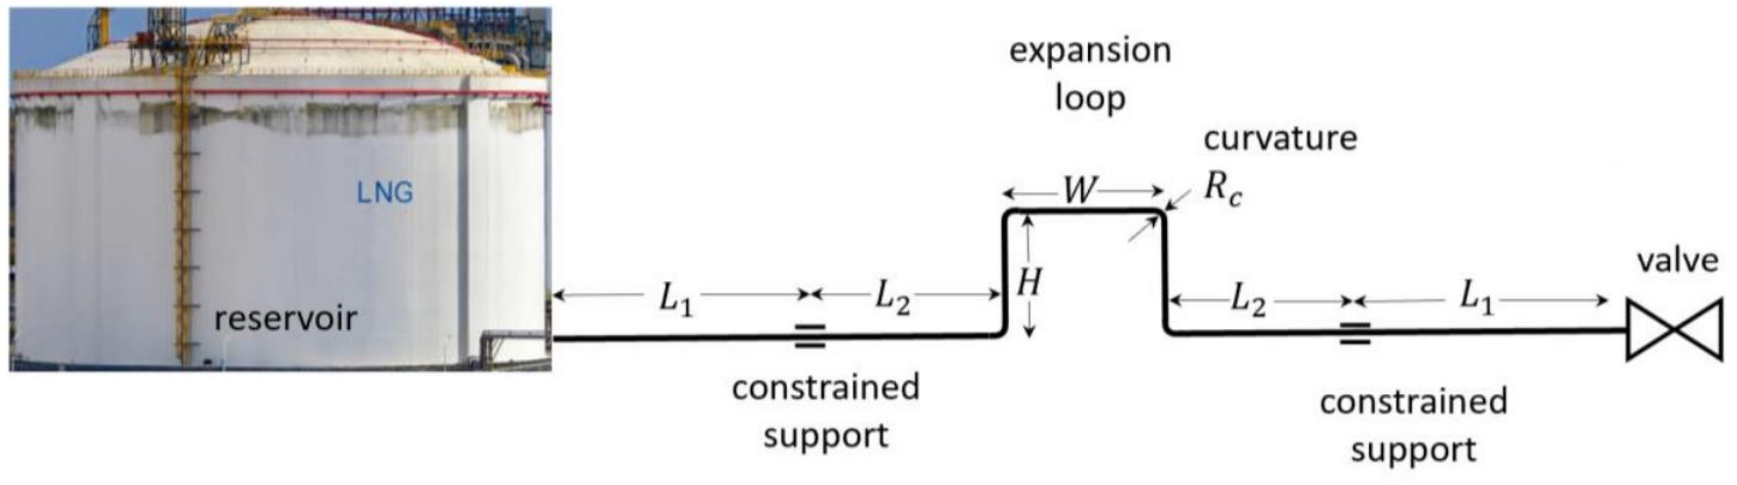
\includegraphics[width = \textwidth]{img/part2a-3.png}
    \caption{3D expansion loop geometry.}
    \label{part2a3}
\end{figure}
The geometry was constructed in ANSYS Discovery. `Fixed supports' were used at the ends of the pipe, and `displacement' supports with fixed y and z displacements were added between $L_1$ and $L_2$, to allow the pipe to move axially in the x direction. The simulation utilised 21 steps and a thermal condition spanning the temperature range was added. Figure \ref{part2a1} shows the deformation at $T = \SI{-160}{\degree C}$ and Figure \ref{part2a2} shows the deformation at $T = \SI{240}{\degree C}$.
\begin{figure}[H]
    \centering
    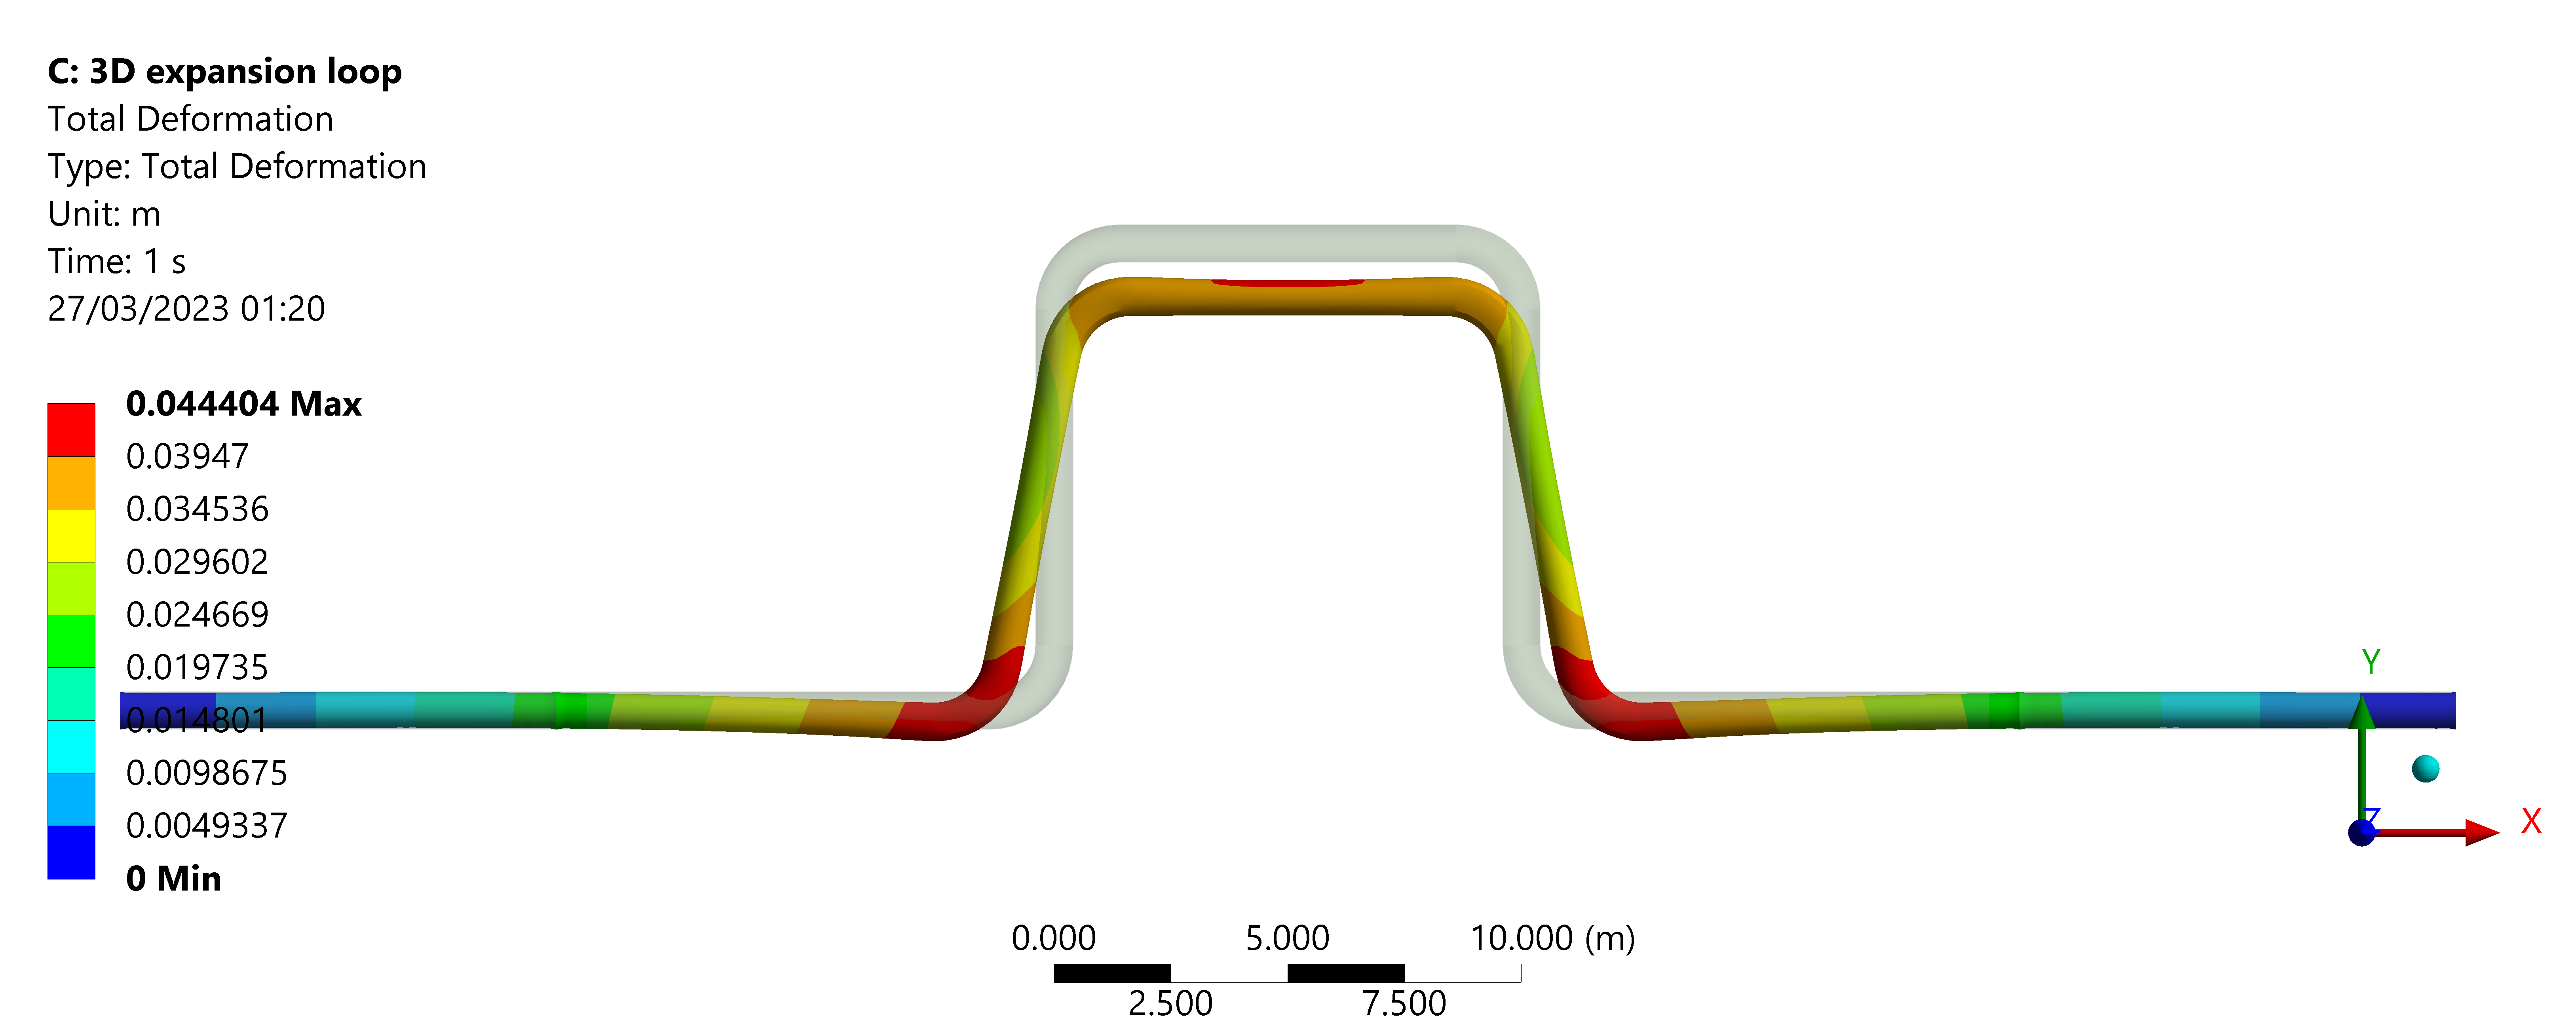
\includegraphics[width = \textwidth]{img/part2a-1.png}
    \caption{3D expansion loop deformation in comparison to undeformed case at $T = \SI{-160}{\degree C}$.}
    \label{part2a1}
\end{figure}
At $T = \SI{-160}{\degree C}$, we see that the expansion loop has contracted and caused the U shape of the loop to be pushed outwards. The bottom pipe bends have deformed the most and have become more obtuse (from \SI{90}{\degree}). Sections $L_2$ has been pushed downwards as a result of the contraction from $L_1$ and the constraints applied, as has section $W$. Sections $H$ have been rotated as a result of the contraction.
\begin{figure}[H]
    \centering
    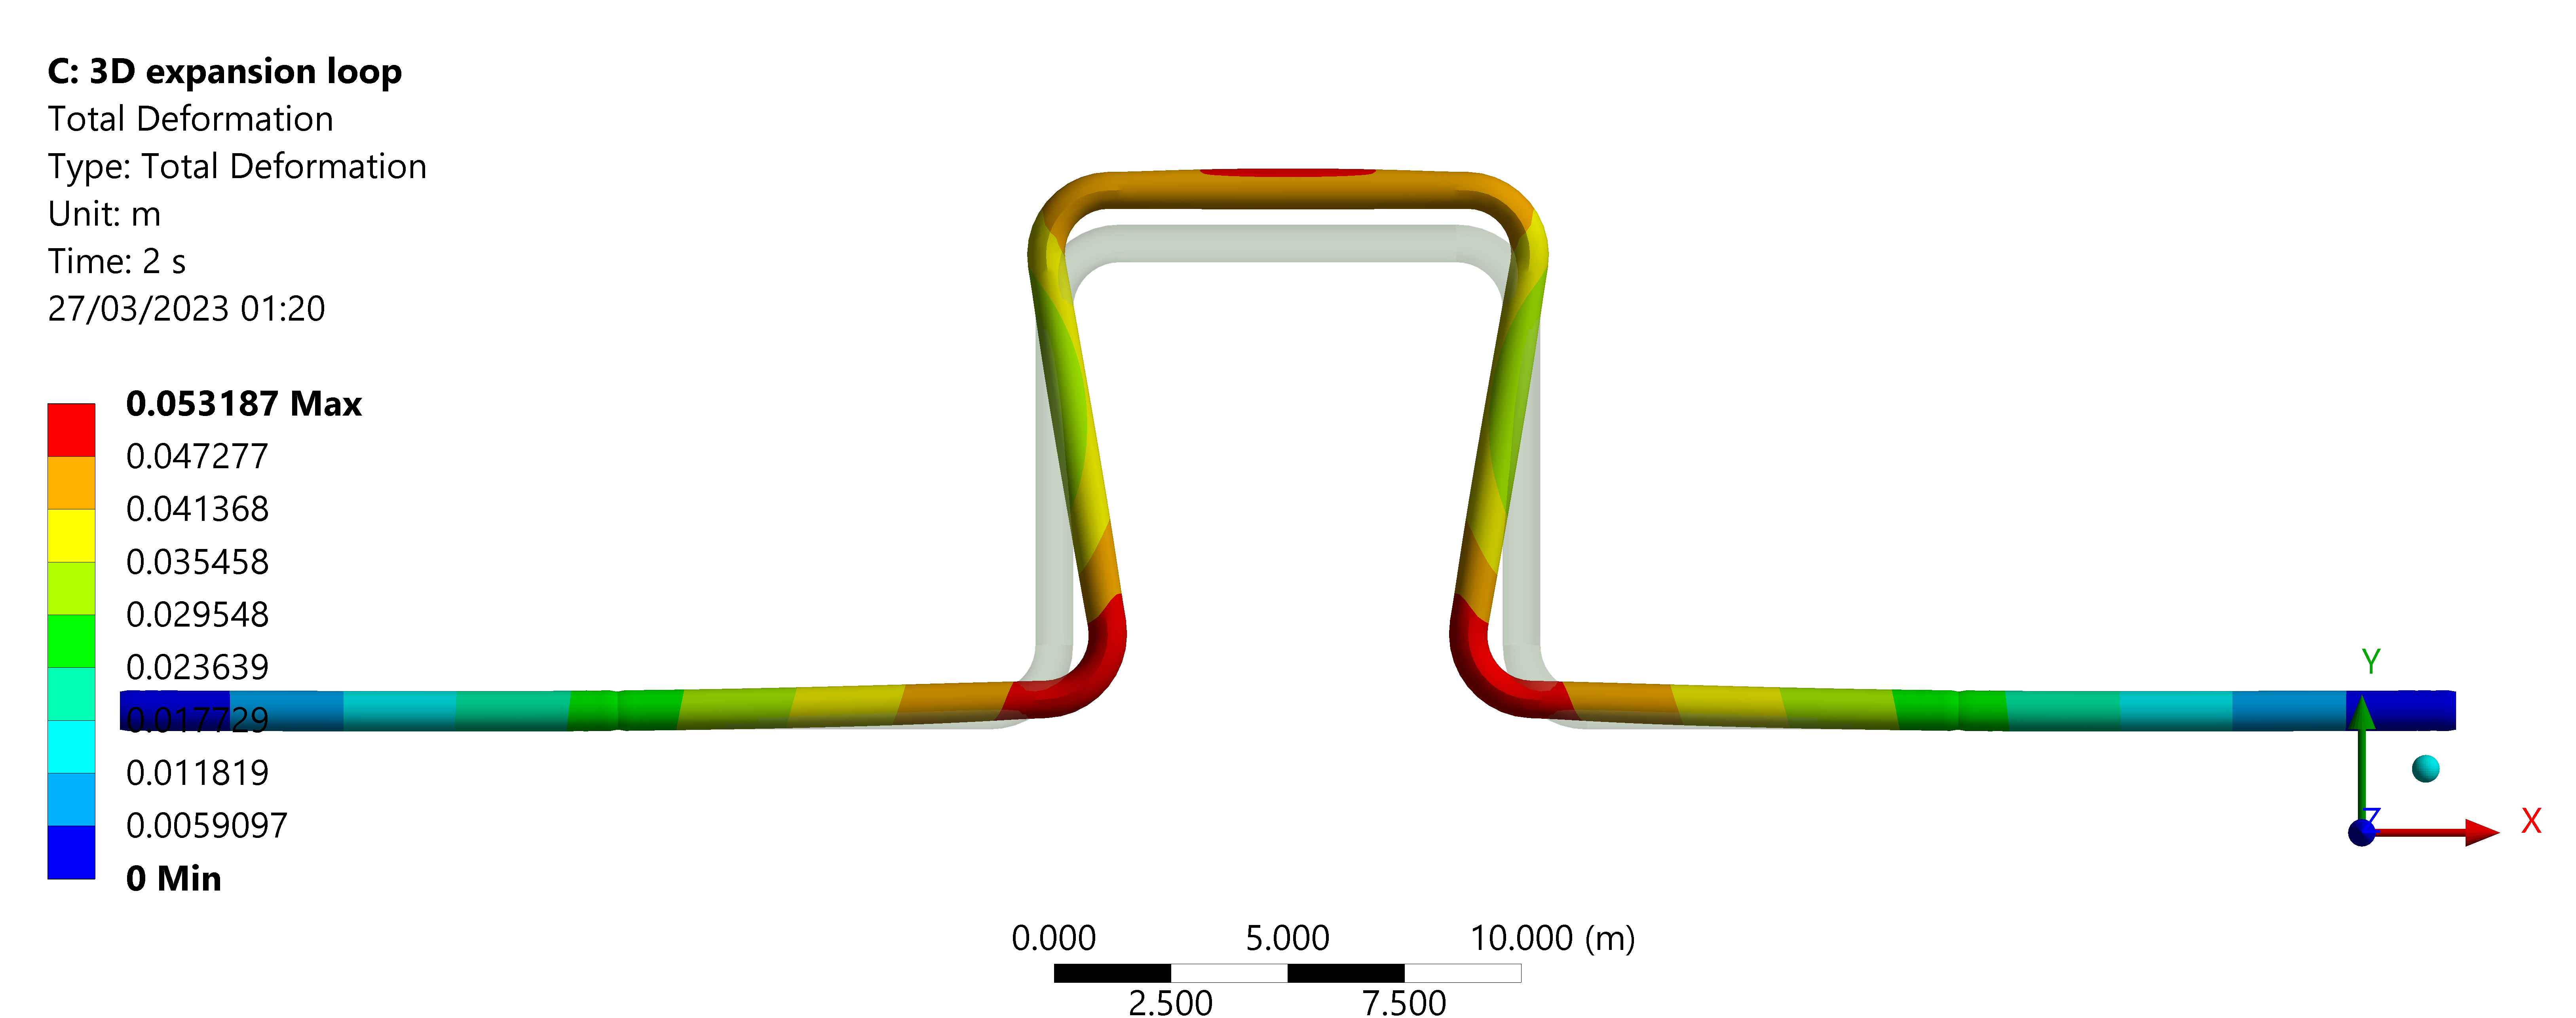
\includegraphics[width = \textwidth]{img/part2a-2.png}
    \caption{3D expansion loop deformation in comparison to undeformed case at $T = \SI{240}{\degree C}$.}
    \label{part2a2}
\end{figure}
At $T = \SI{240}{\degree C}$, we see that the expansion loop has expanded and caused the U shape of the loop to be pushed inwards. The bottom pipe bends have again deformed the most and have become acute. Sections $L_2$ have been pushed upwards slightly as a result of the expansion of $L_1$ and the constraints applied. Section $W$ has been pushed upward as a result of the expansion and sections $H$ have been rotated as a result of the expansion.

Thermoelastic stress is dependent on the material's thermal expansion coefficient, which is a measure of how much the material will expand or contract in response to temperature changes. It is also dependent on the magnitude and rate of temperature change (something not captured in ANSYS Static Structural), as well as the geometry and boundary conditions of the material.

If the temperature change is rapid or significant, the resulting thermoelastic stress can be high and potentially cause damage or failure in the material. However, if the temperature change is gradual and within the material's design limits, the resulting thermoelastic stress can be controlled and beneficial for certain applications, such as this.

Understanding thermoelastic stress is crucial for designing materials and structures that can withstand temperature changes and avoid failure due to stress and deformation.
\subsection{Plot of variation of maximum displacement of pipe bends}
The pipe bend surfaces were indexed in the analysis, and the component deformations in the x and y axes were found. The maximum displacements from each time step were plotted in MATLAB. Figures \ref{part2b1}, \ref{part2b2} show the deformations in x and y axis respectively.
\begin{figure}[H]
    \centering
    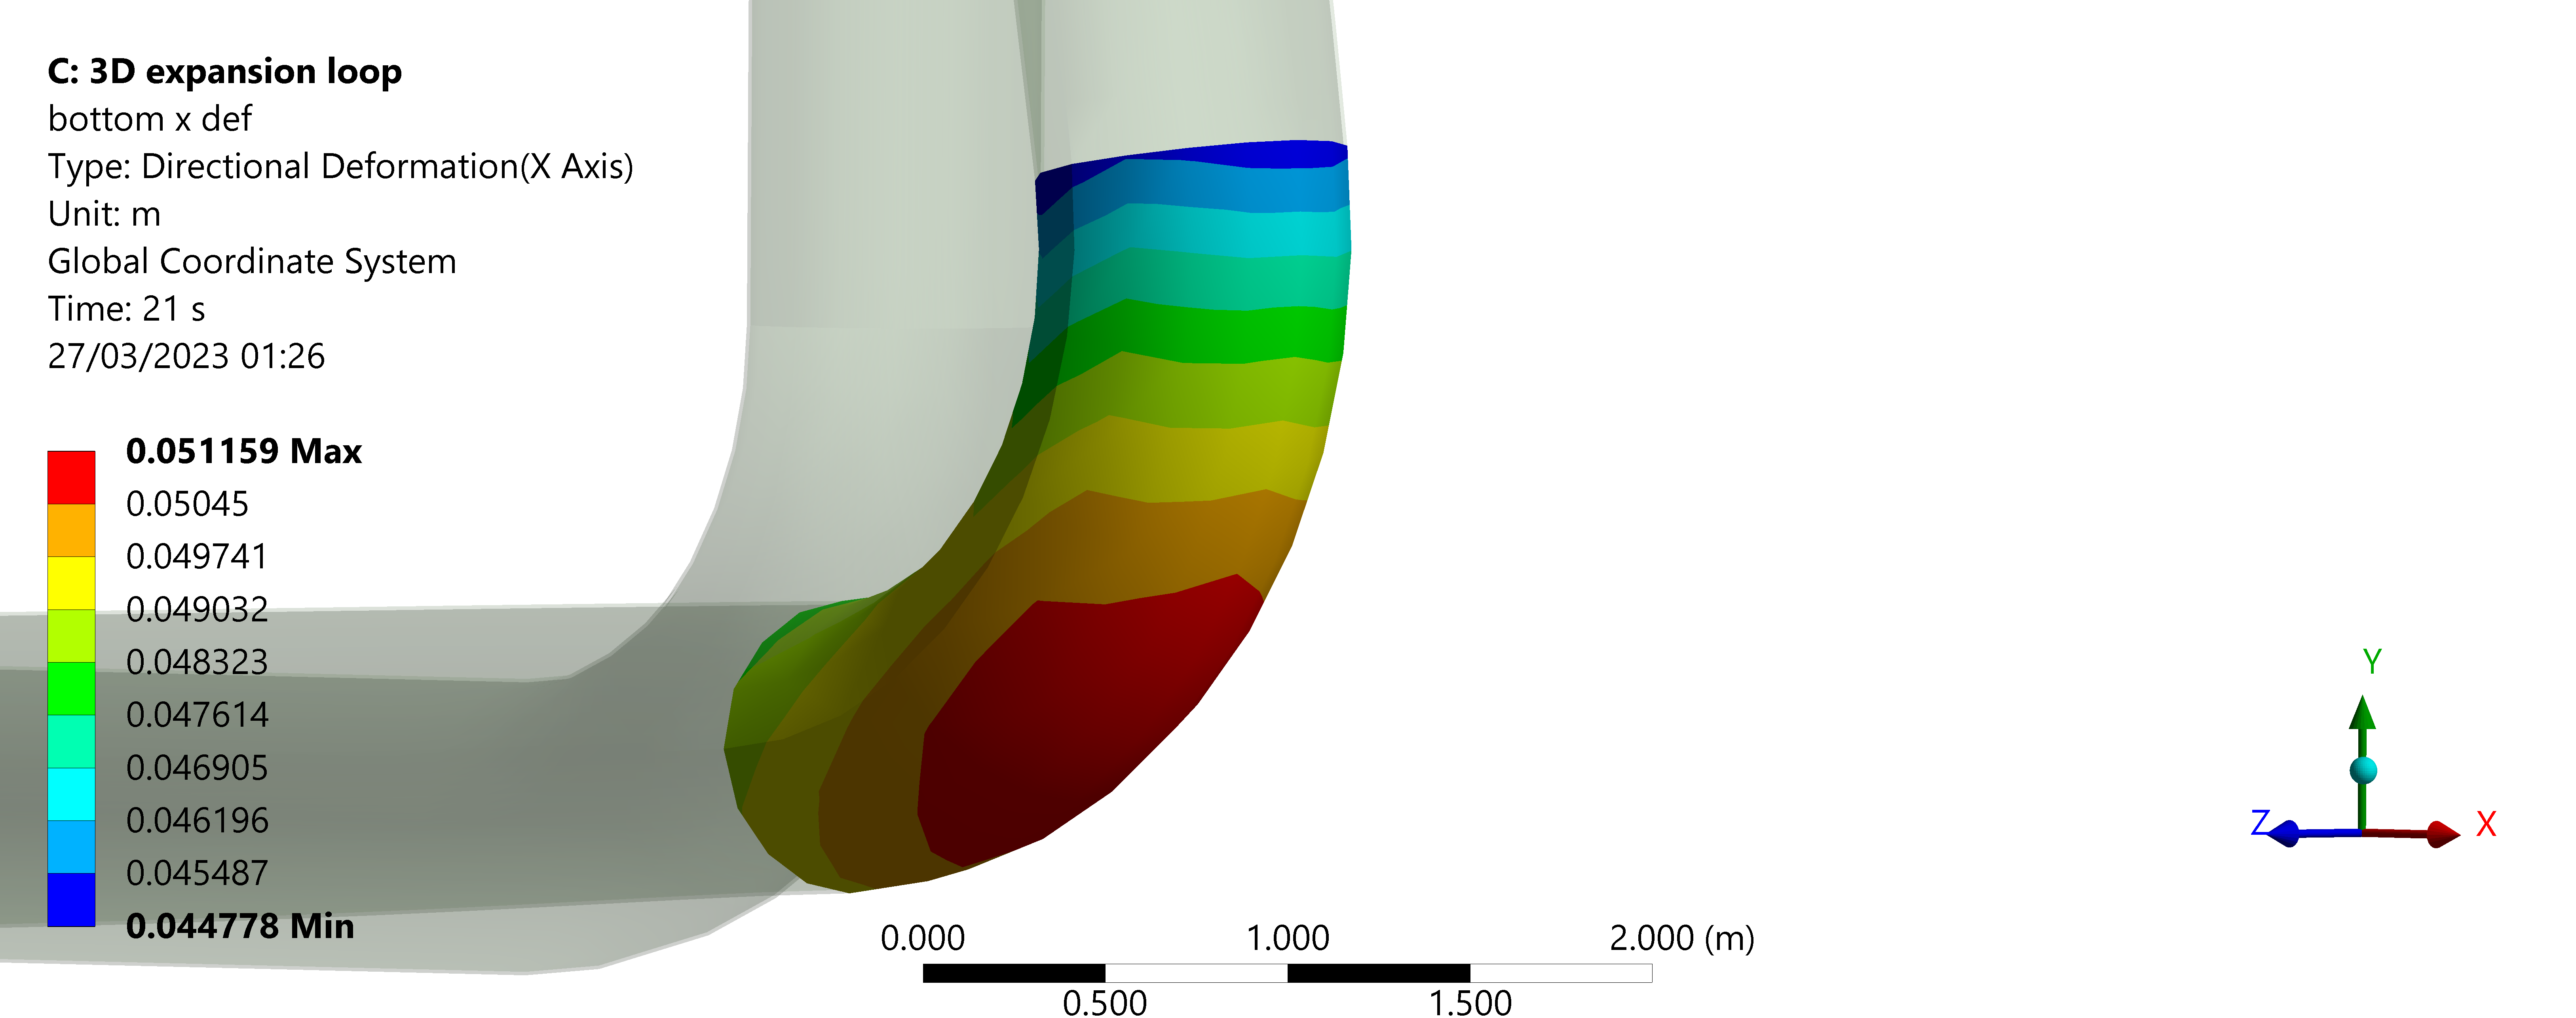
\includegraphics[width = \textwidth]{img/part2b-1.png}
    \caption{ANSYS maximum deformation in x-axis at time step 21, $T-T_0 = \SI{218}{\degree C}$, bottom pipe bend.}
    \label{part2b1}
\end{figure}
\begin{figure}[H]
    \centering
    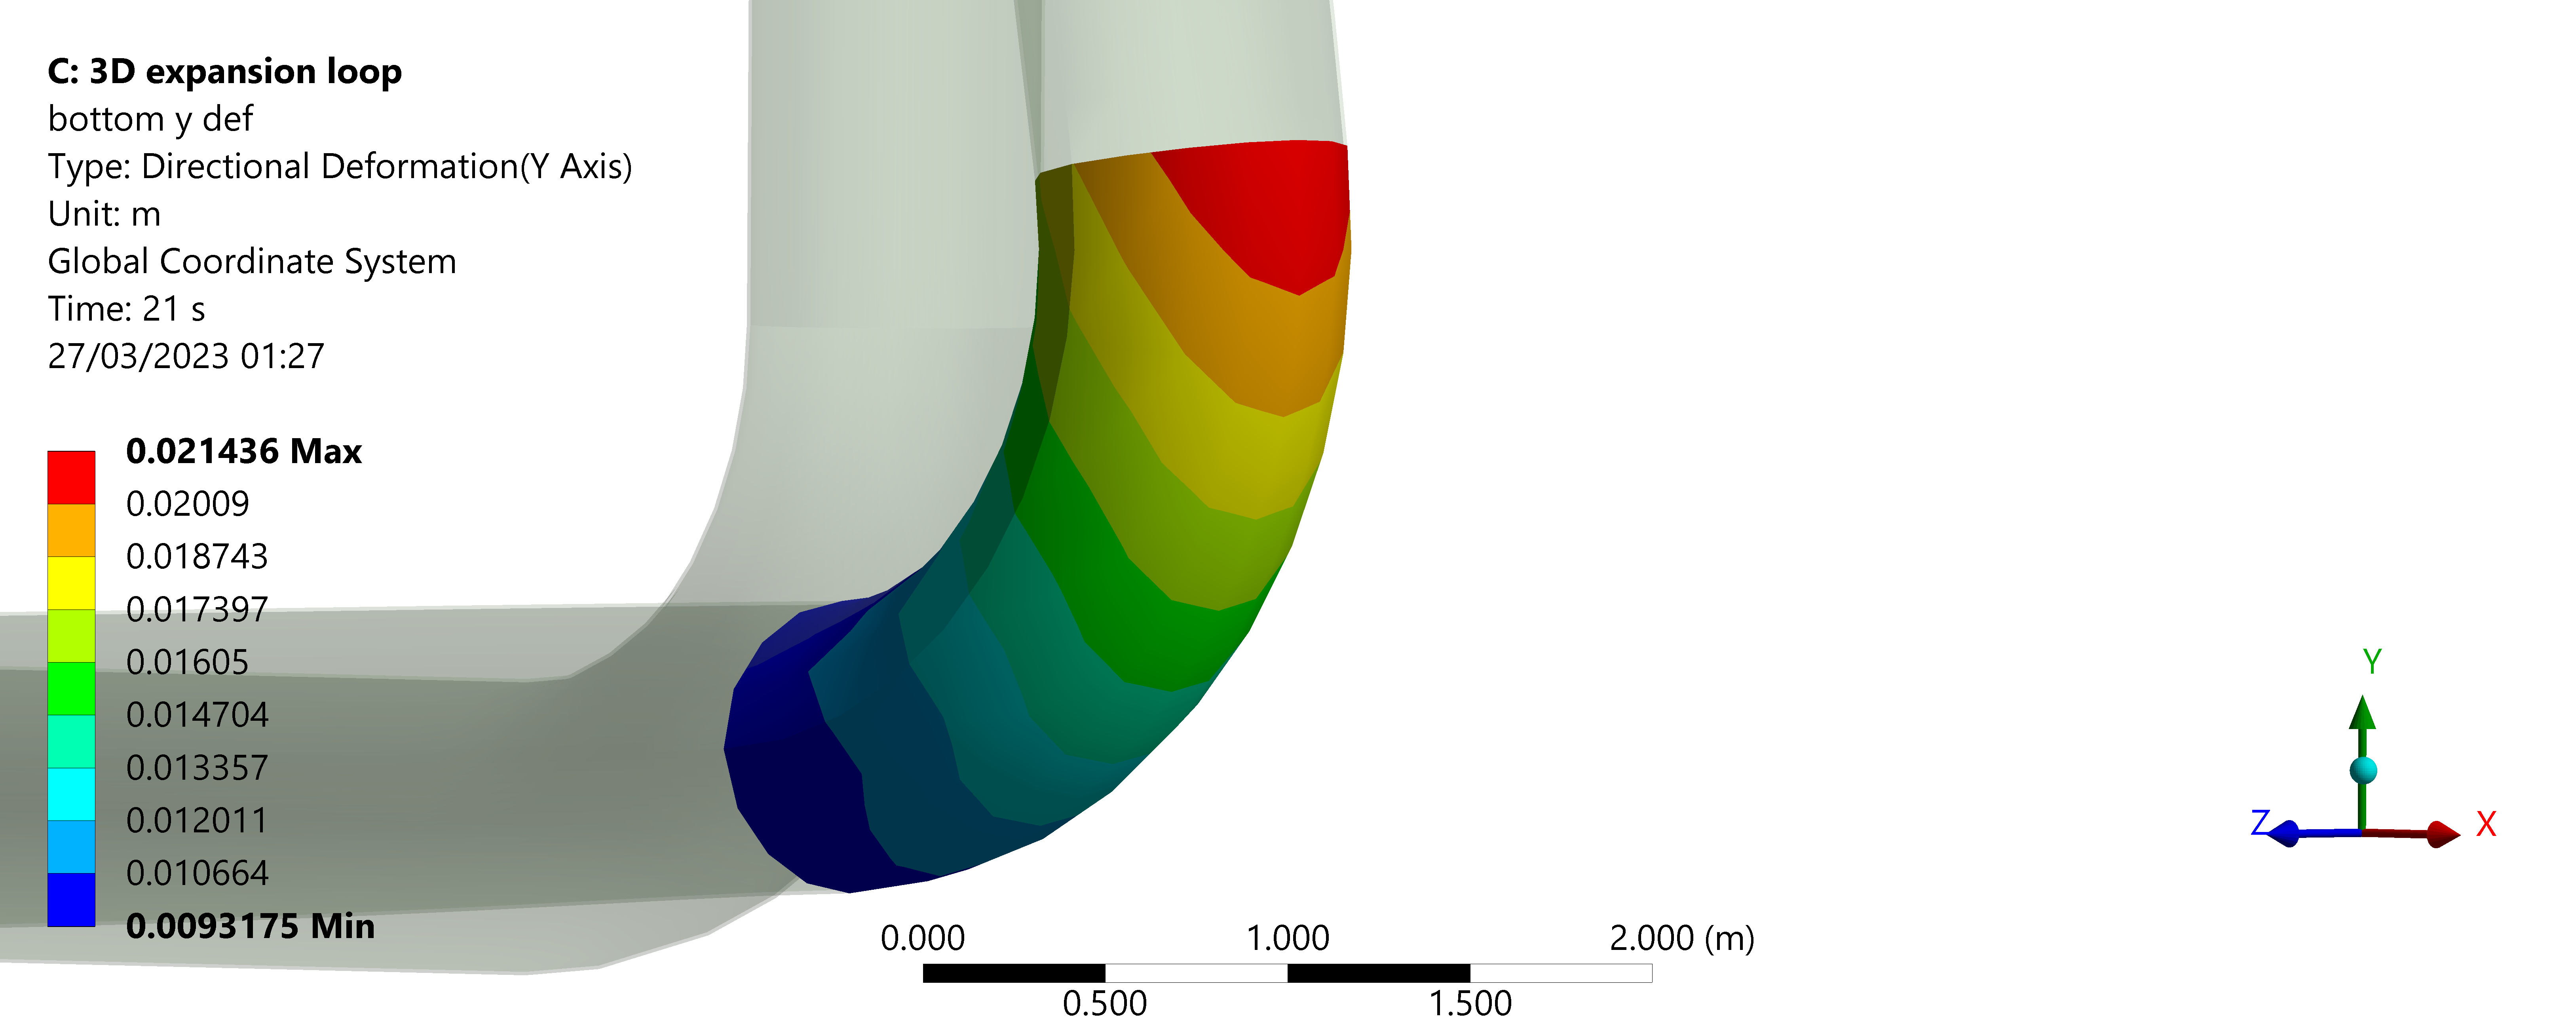
\includegraphics[width = \textwidth]{img/part2b-2.png}
    \caption{ANSYS maximum deformation in y-axis at time step 21, $T-T_0 = \SI{218}{\degree C}$, bottom pipe bend.}
    \label{part2b2}
\end{figure}
Figure \ref{part2b3} shows a comparison in the location of the maximum deformation between the first time step and the last. We see that the point of maximum deformation is the apex of the outside bend of the pipe. This appears to be consistent throughout all the time steps in the analysis. Another point of major deformation is the connection point between the bend and the vertical section of the loop. One problem that arises is ANSYS gives us the smallest deformation as maximum for negative results and the largest deformation for positive results. Usually, this is not an issue as we can average between maximum and minimum. However, for the interest in consistency, the node at which maximum displacement occurs in all time steps was selected to index results, to avoid the issue of different parts of the surface being indexed as `maximum' deformation. The node selected for the bottom bend is shown in Figure \ref{part2b4} and a similarly placed node (at the point of maximum deformation) was chosen for the top bend. The results were indexed for one half of the loop (left side), as the loop is symmetrical.
\begin{figure}[H]
    \centering
    \begin{subfigure}[b]{0.45\textwidth}
        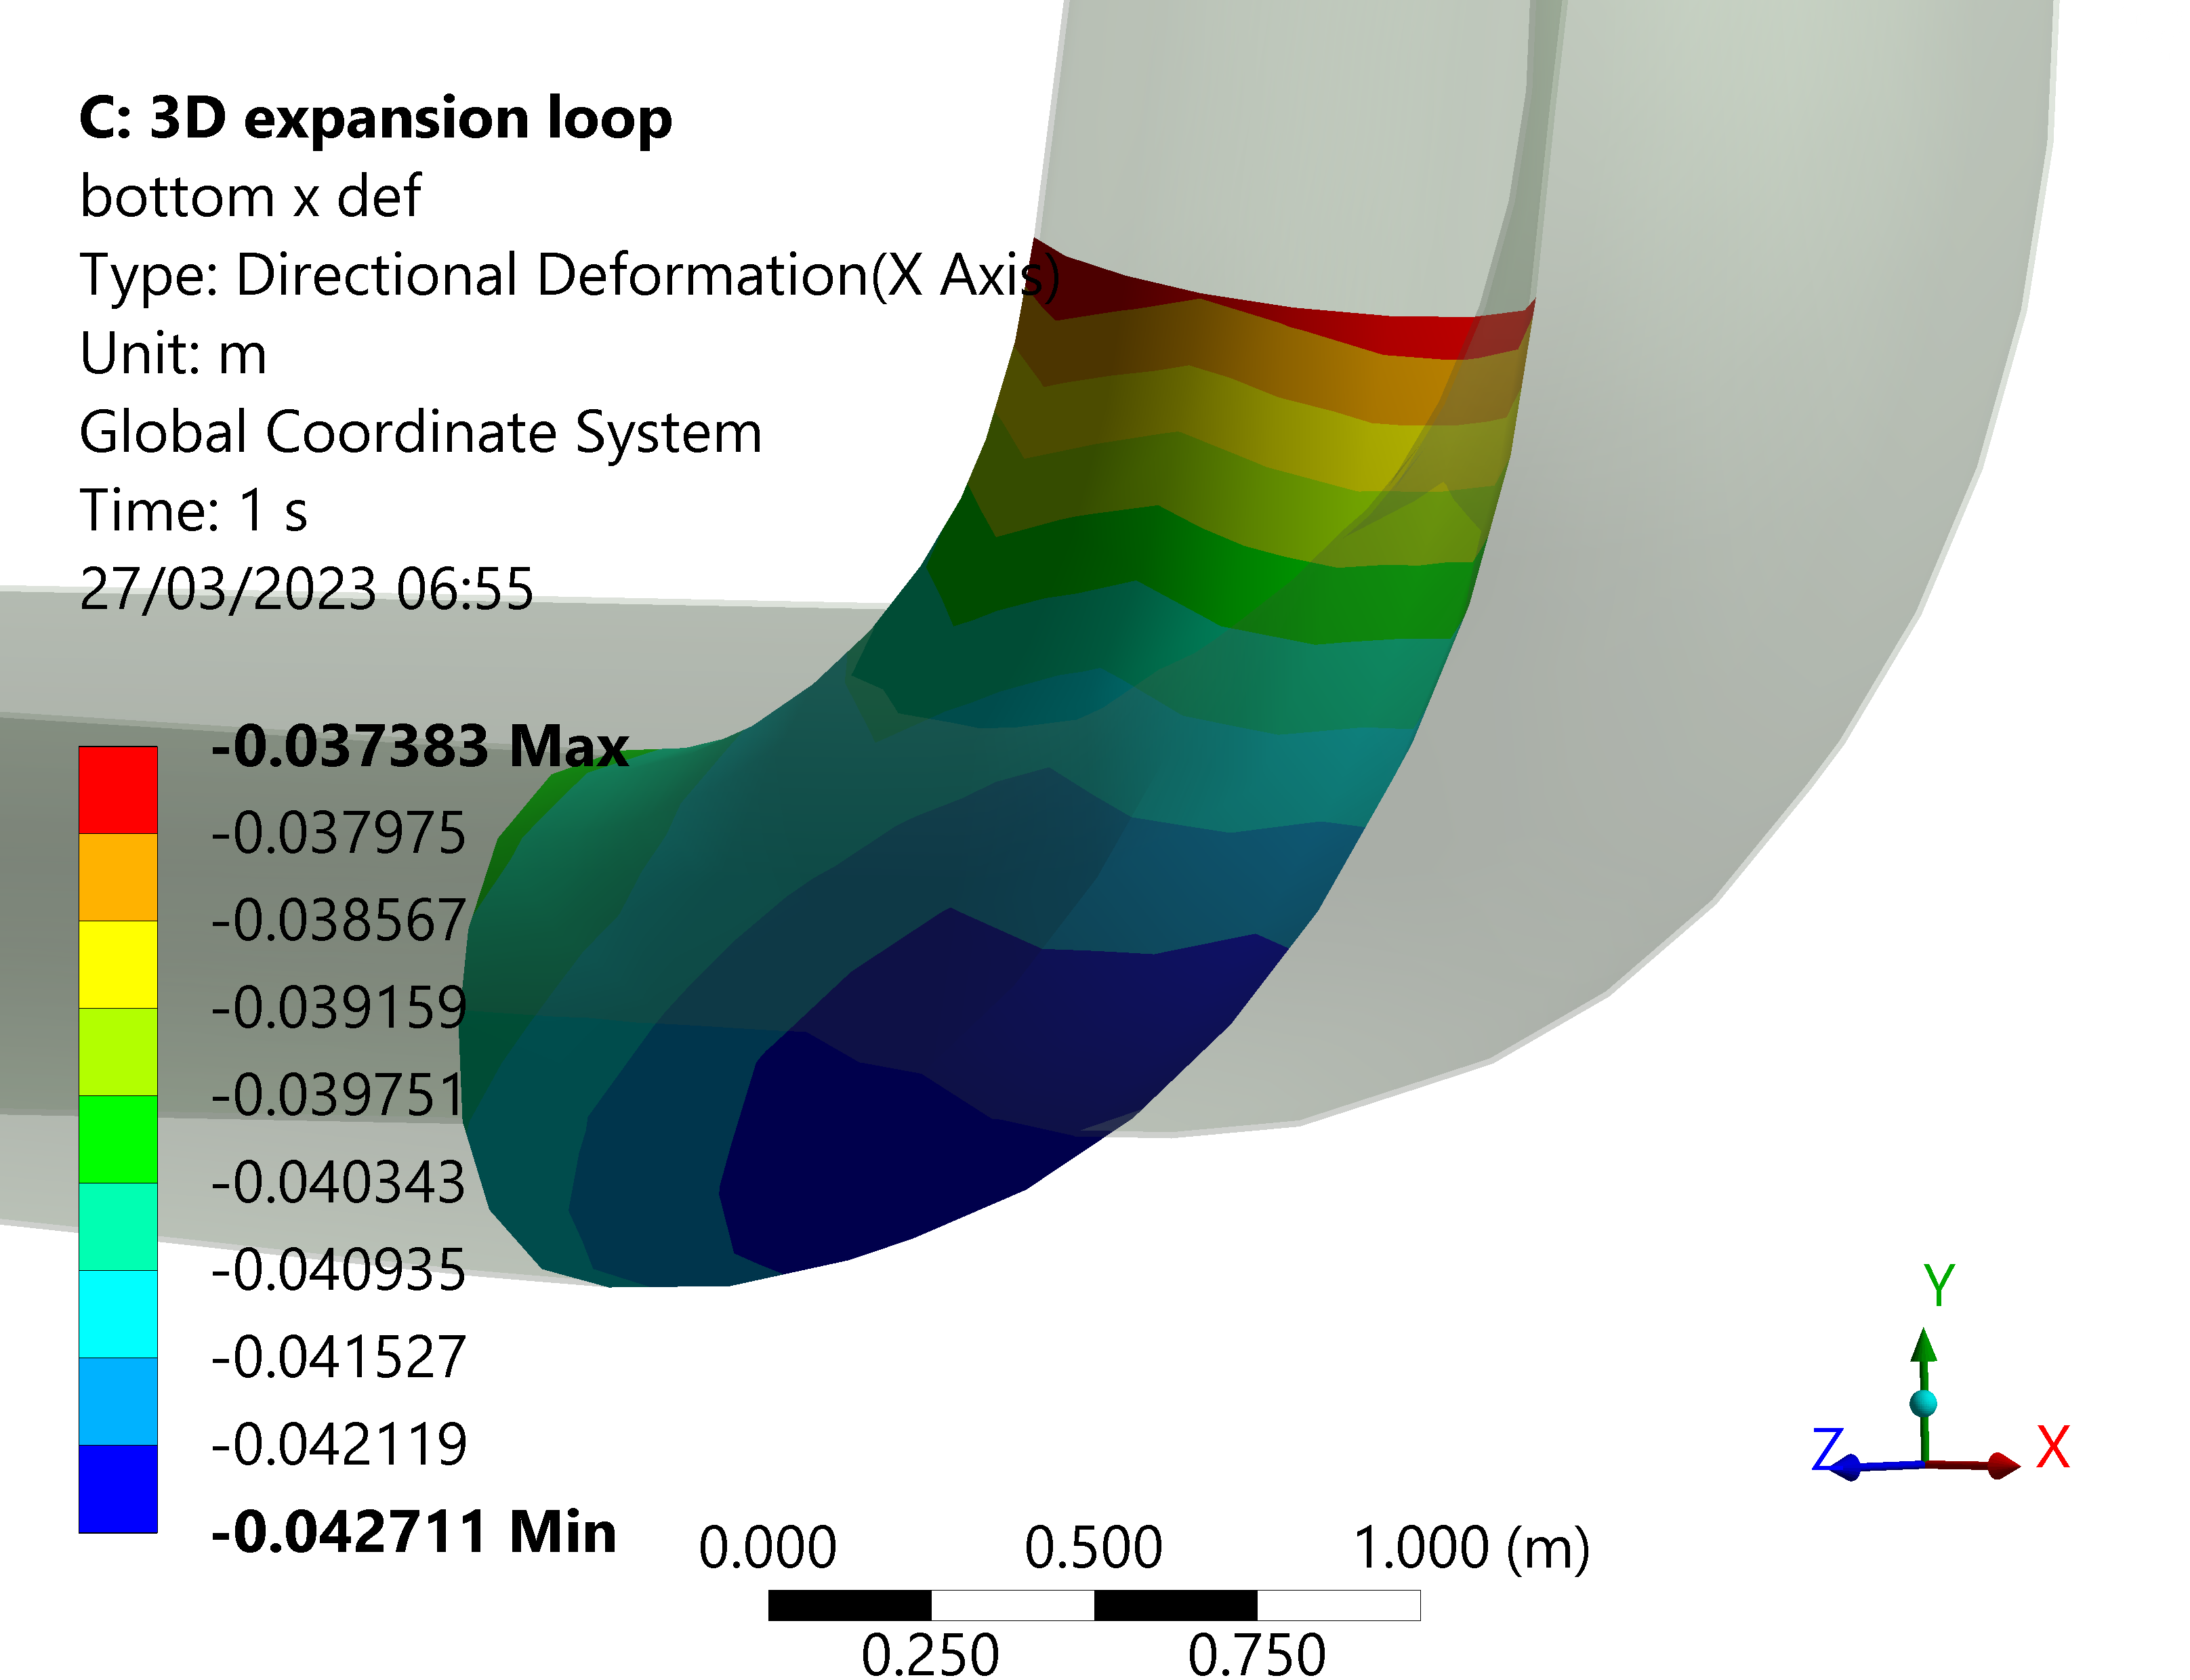
\includegraphics[width=\textwidth]{img/part2b-3.png}
    \end{subfigure}
    \hfill
    \begin{subfigure}[b]{0.45\textwidth}
        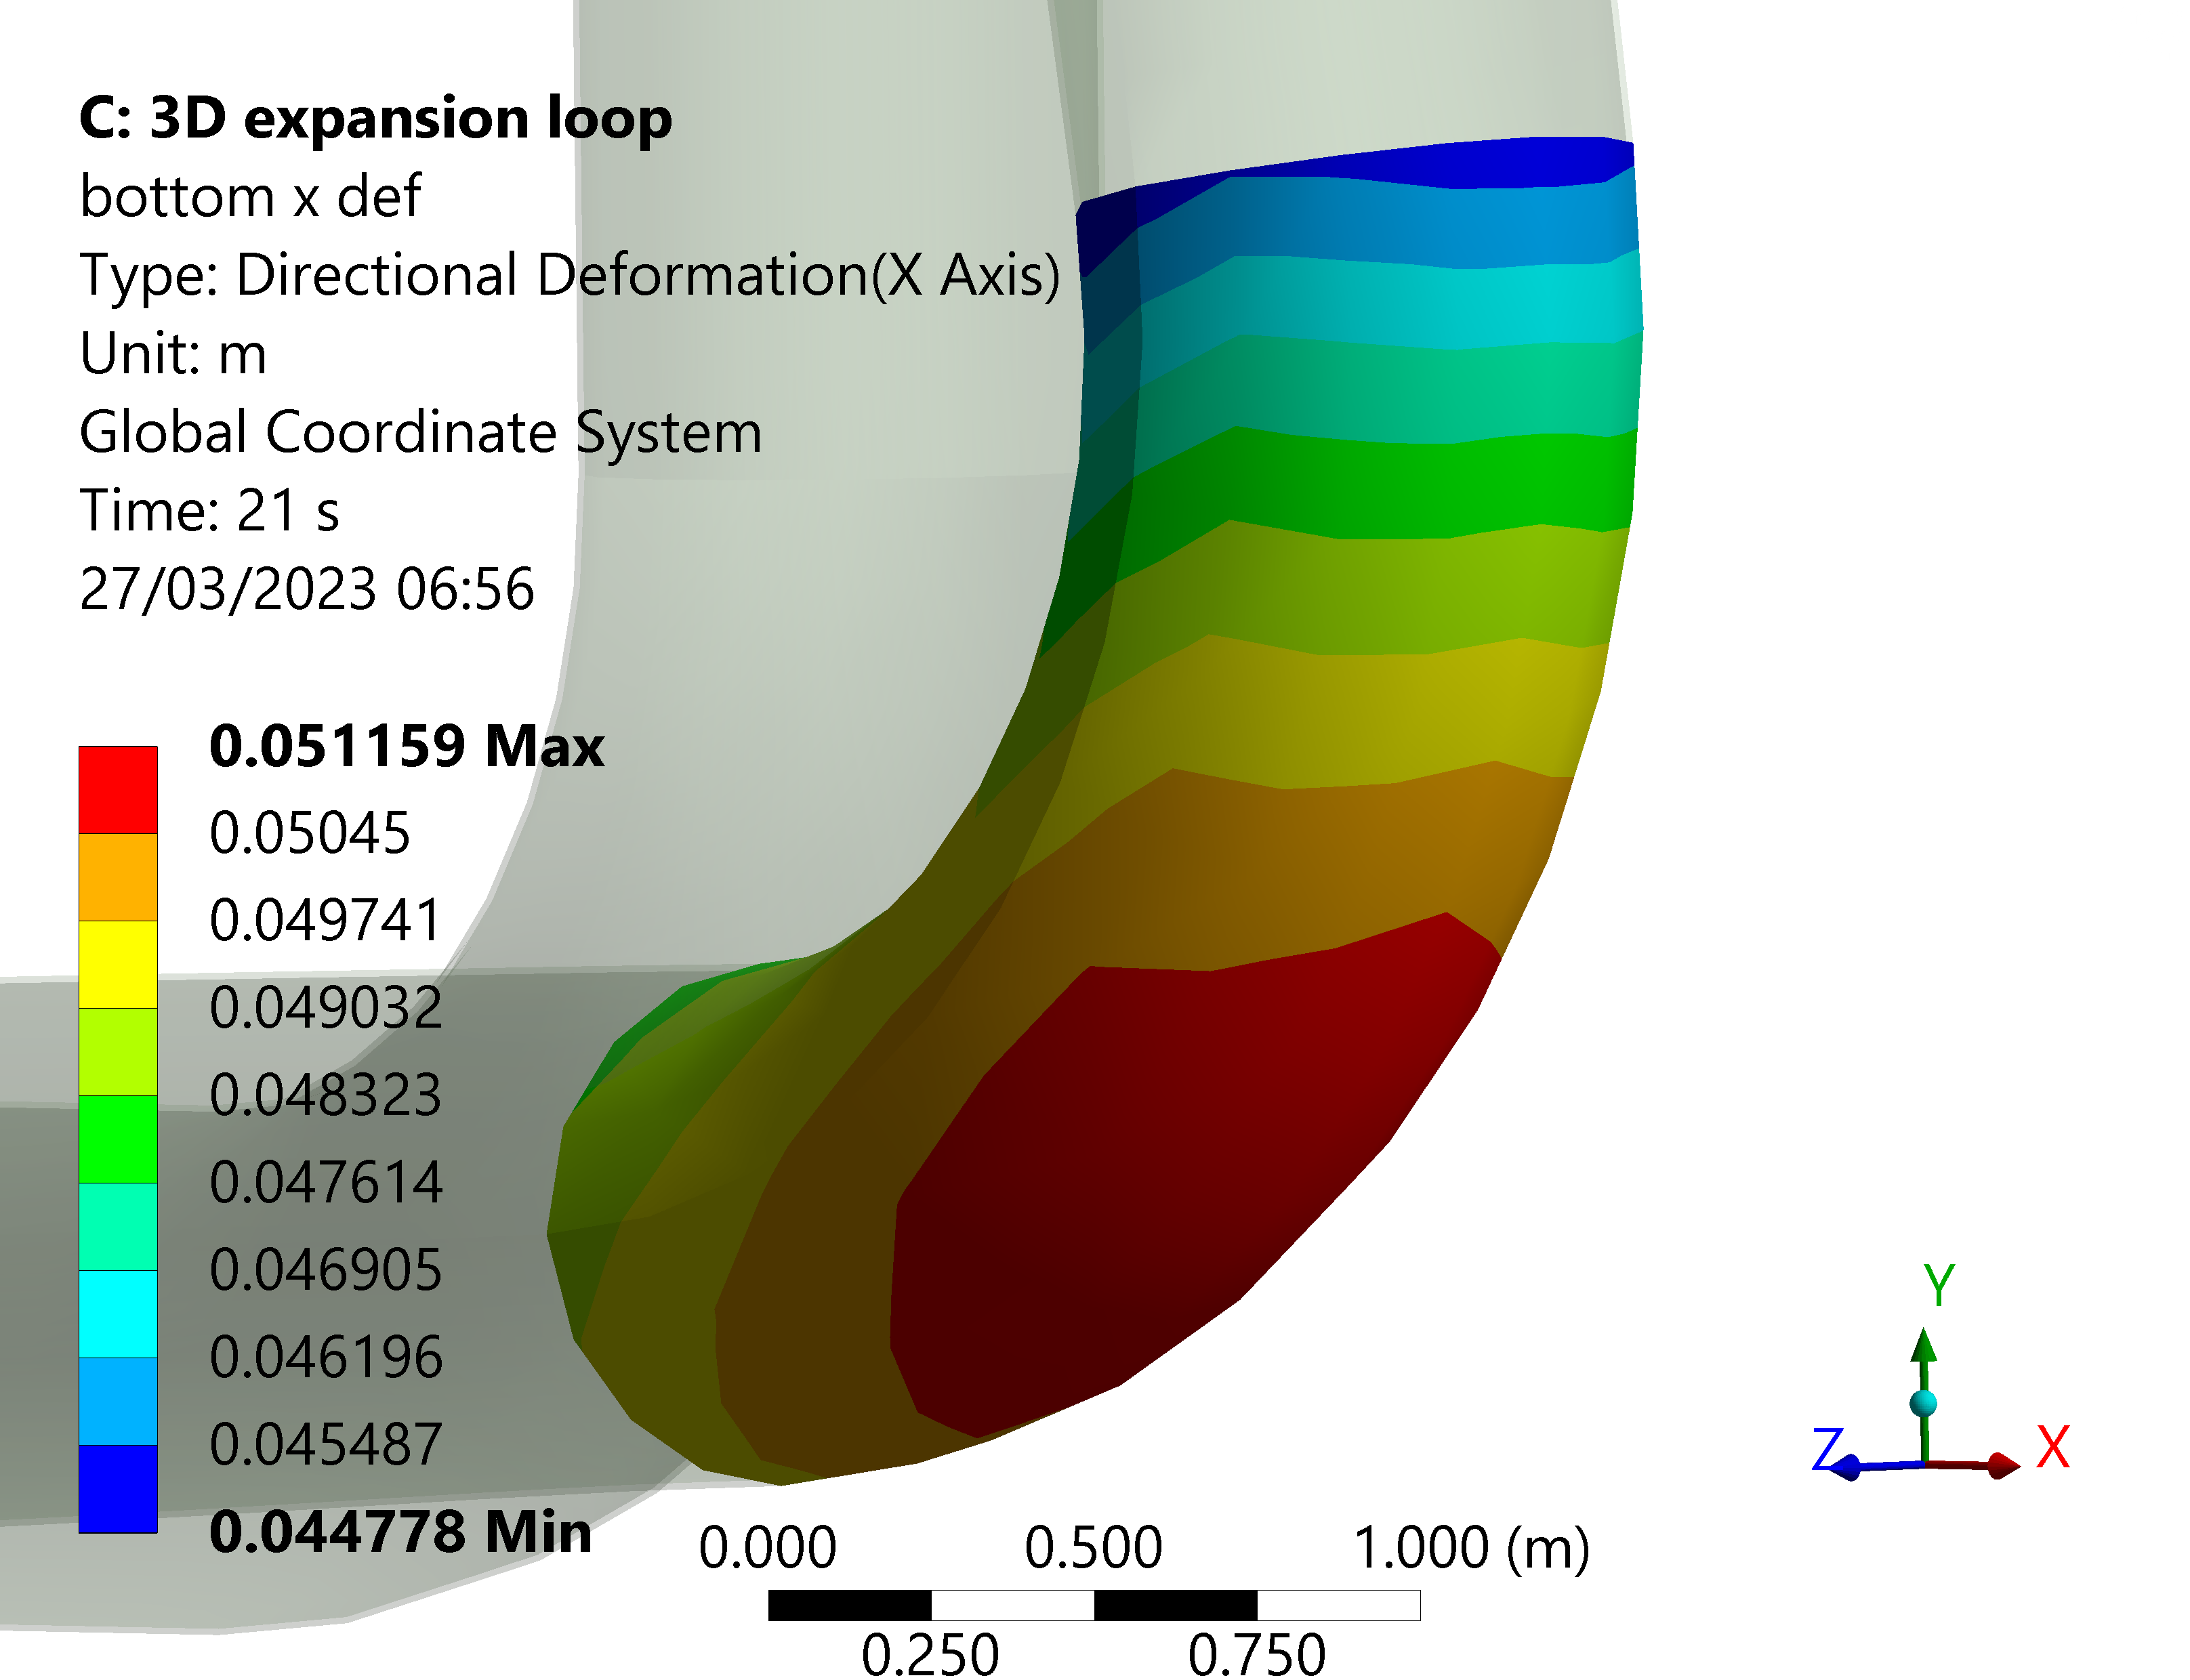
\includegraphics[width=\textwidth]{img/part2b-4.png}
    \end{subfigure}
    \caption{ANSYS maximum deformation in x-axis at time step 1 and 21, $T-T_0 = \SI{-188}{\degree C}-\SI{218}{\degree C}$, bottom pipe bend.}
    \label{part2b3}
\end{figure}
\begin{figure}[H]
    \centering
    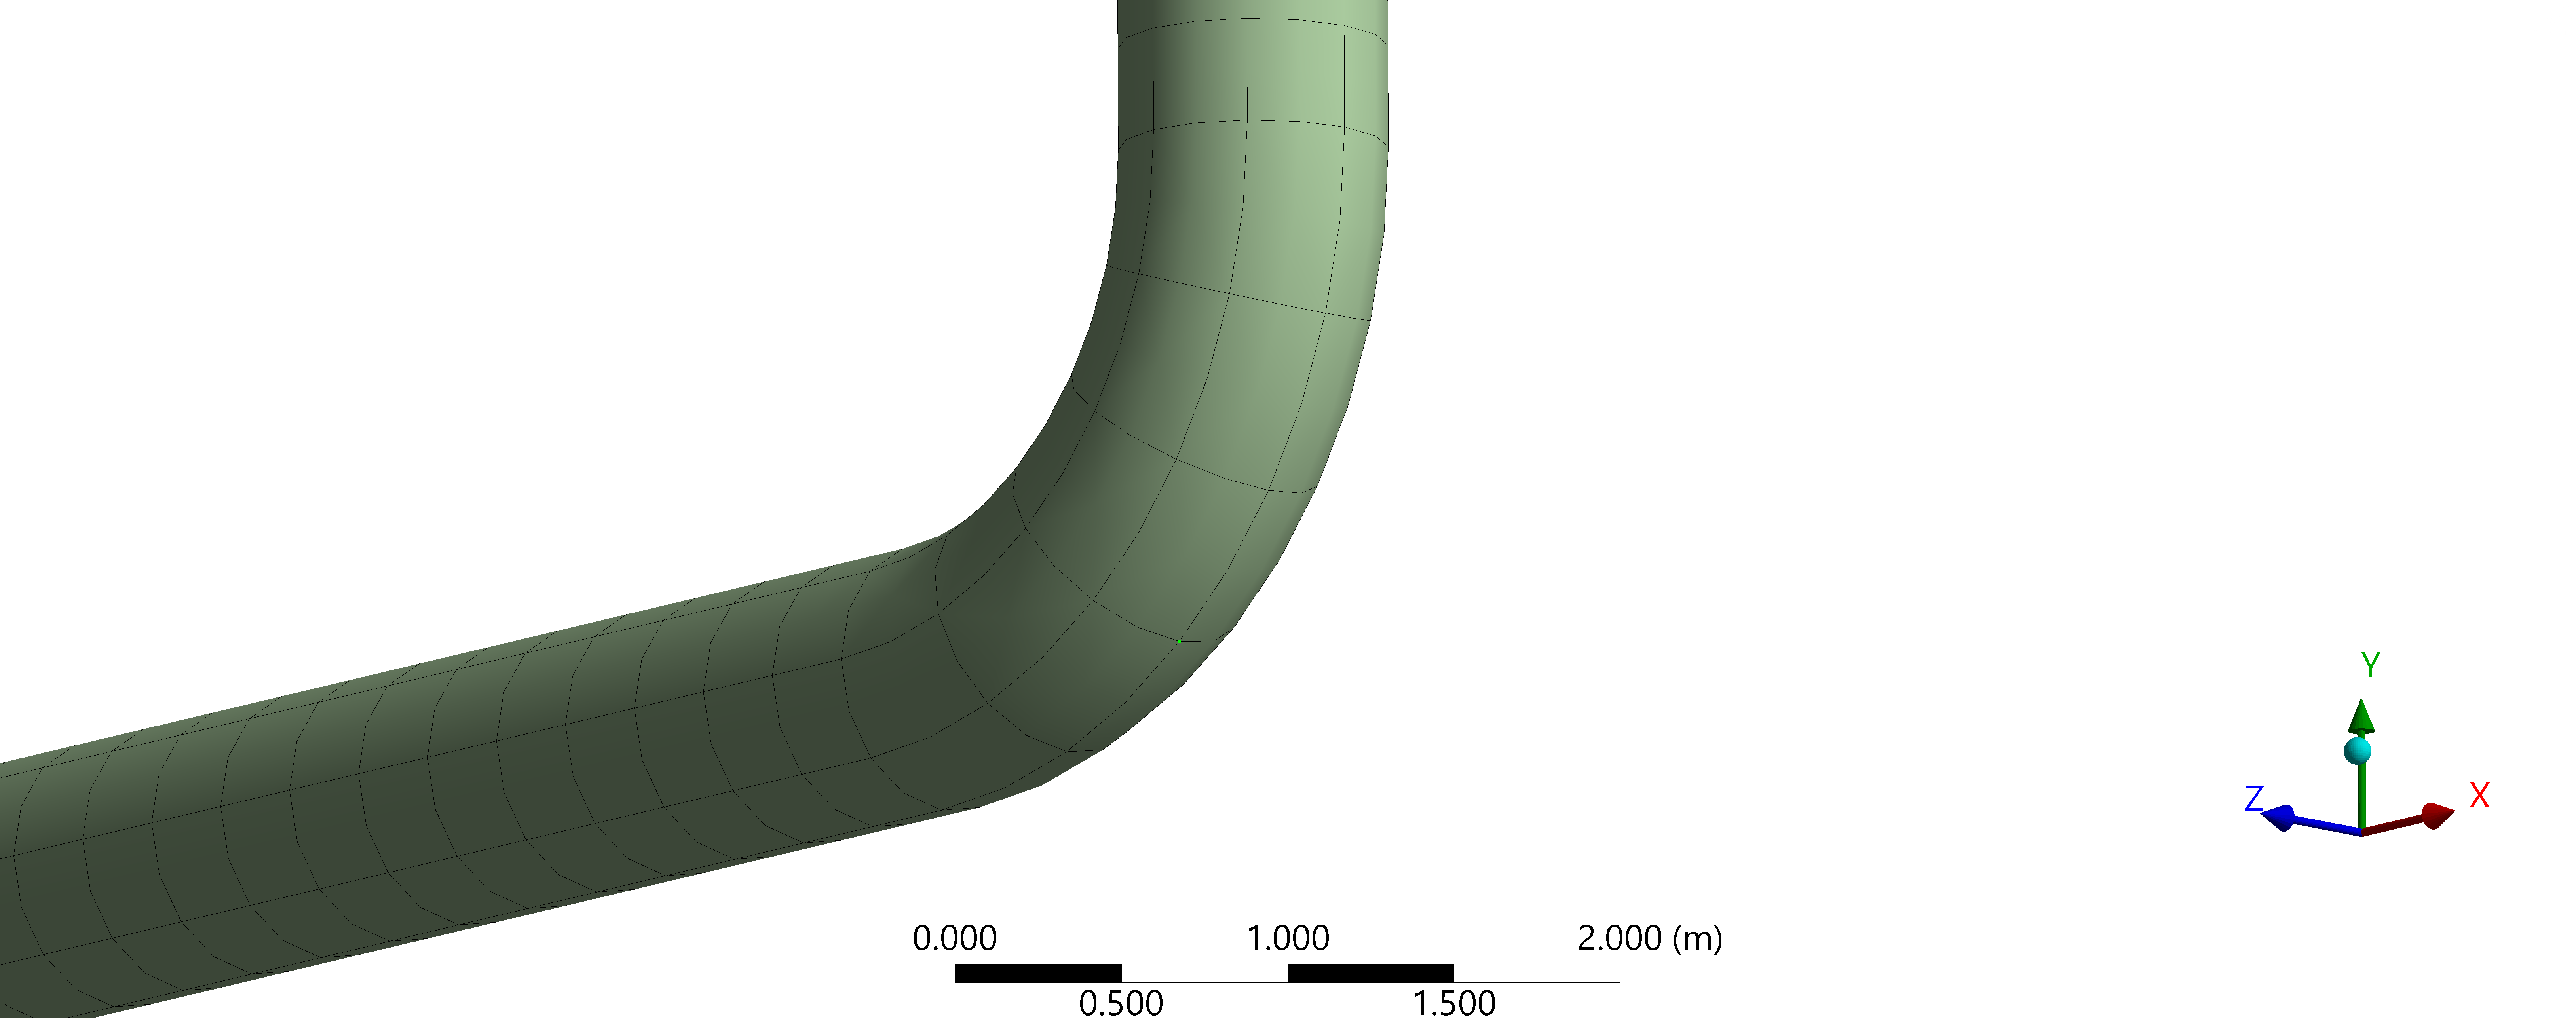
\includegraphics[width = 0.8\textwidth]{img/part2b-5.png}
    \caption{Node selected for pipe bend analysis.}
    \label{part2b4}
\end{figure}
\begin{figure}[H]
    \centering
    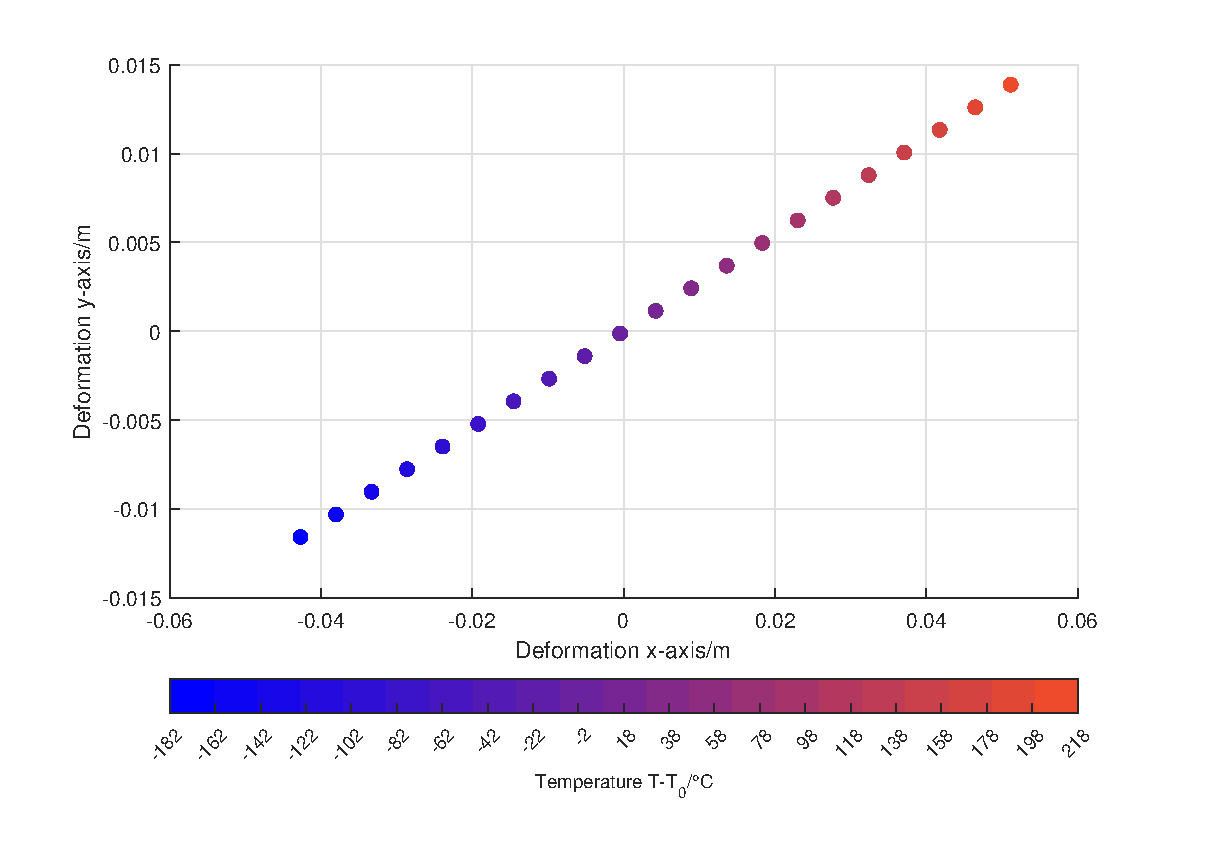
\includegraphics[width = 0.8\textwidth]{img/part2bi.eps}
    \caption{Plot to show maximum displacement of bottom pipe bend at node of maximum displacement.}
    \label{part2b5}
\end{figure}
\begin{figure}[H]
    \centering
    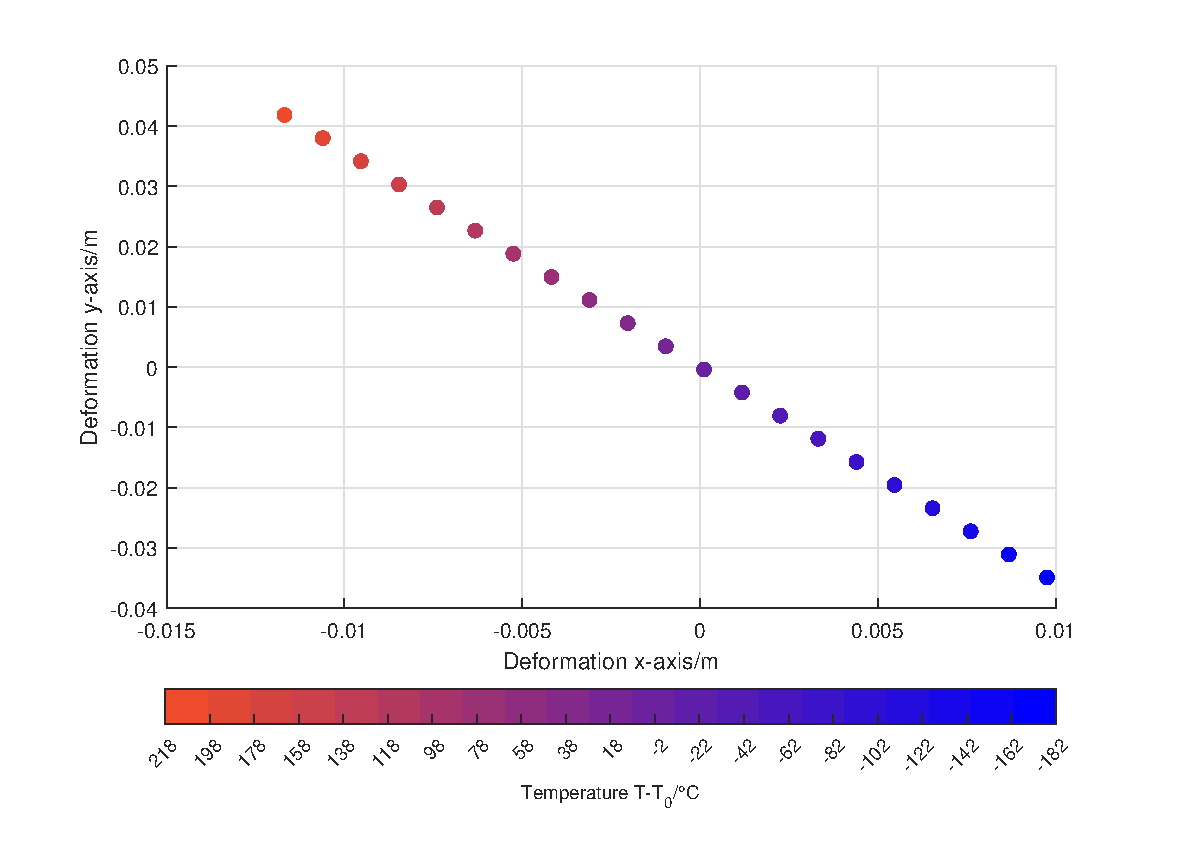
\includegraphics[width = 0.8\textwidth]{img/part2bii.eps}
    \caption{Plot to show maximum displacement of top pipe bend at node of maximum displacement.}
    \label{part2b6}
\end{figure}
The plots show a linear deformation. Note that the deformation in the x-axis is less overall than in the y-axis in Figure \ref{part2b5} (bottom bend) and this is the opposite in Figure \ref{part2b6} (top bend).
\subsection{Plot of variation of maximum stress of pipe bends}
The maximum principal stress was indexed in the results from ANSYS. This was then plotted in Figure \ref{part2c1}. The maximum shear stress was also indexed and plotted alongside the maximum principal stress in Figure \ref{part2c2}. The results show that the maximum principal stress occurs in the top bend of the pipe on the lateral edges, as shown in Figure \ref{part2c3}
\begin{figure}[H]
    \centering
    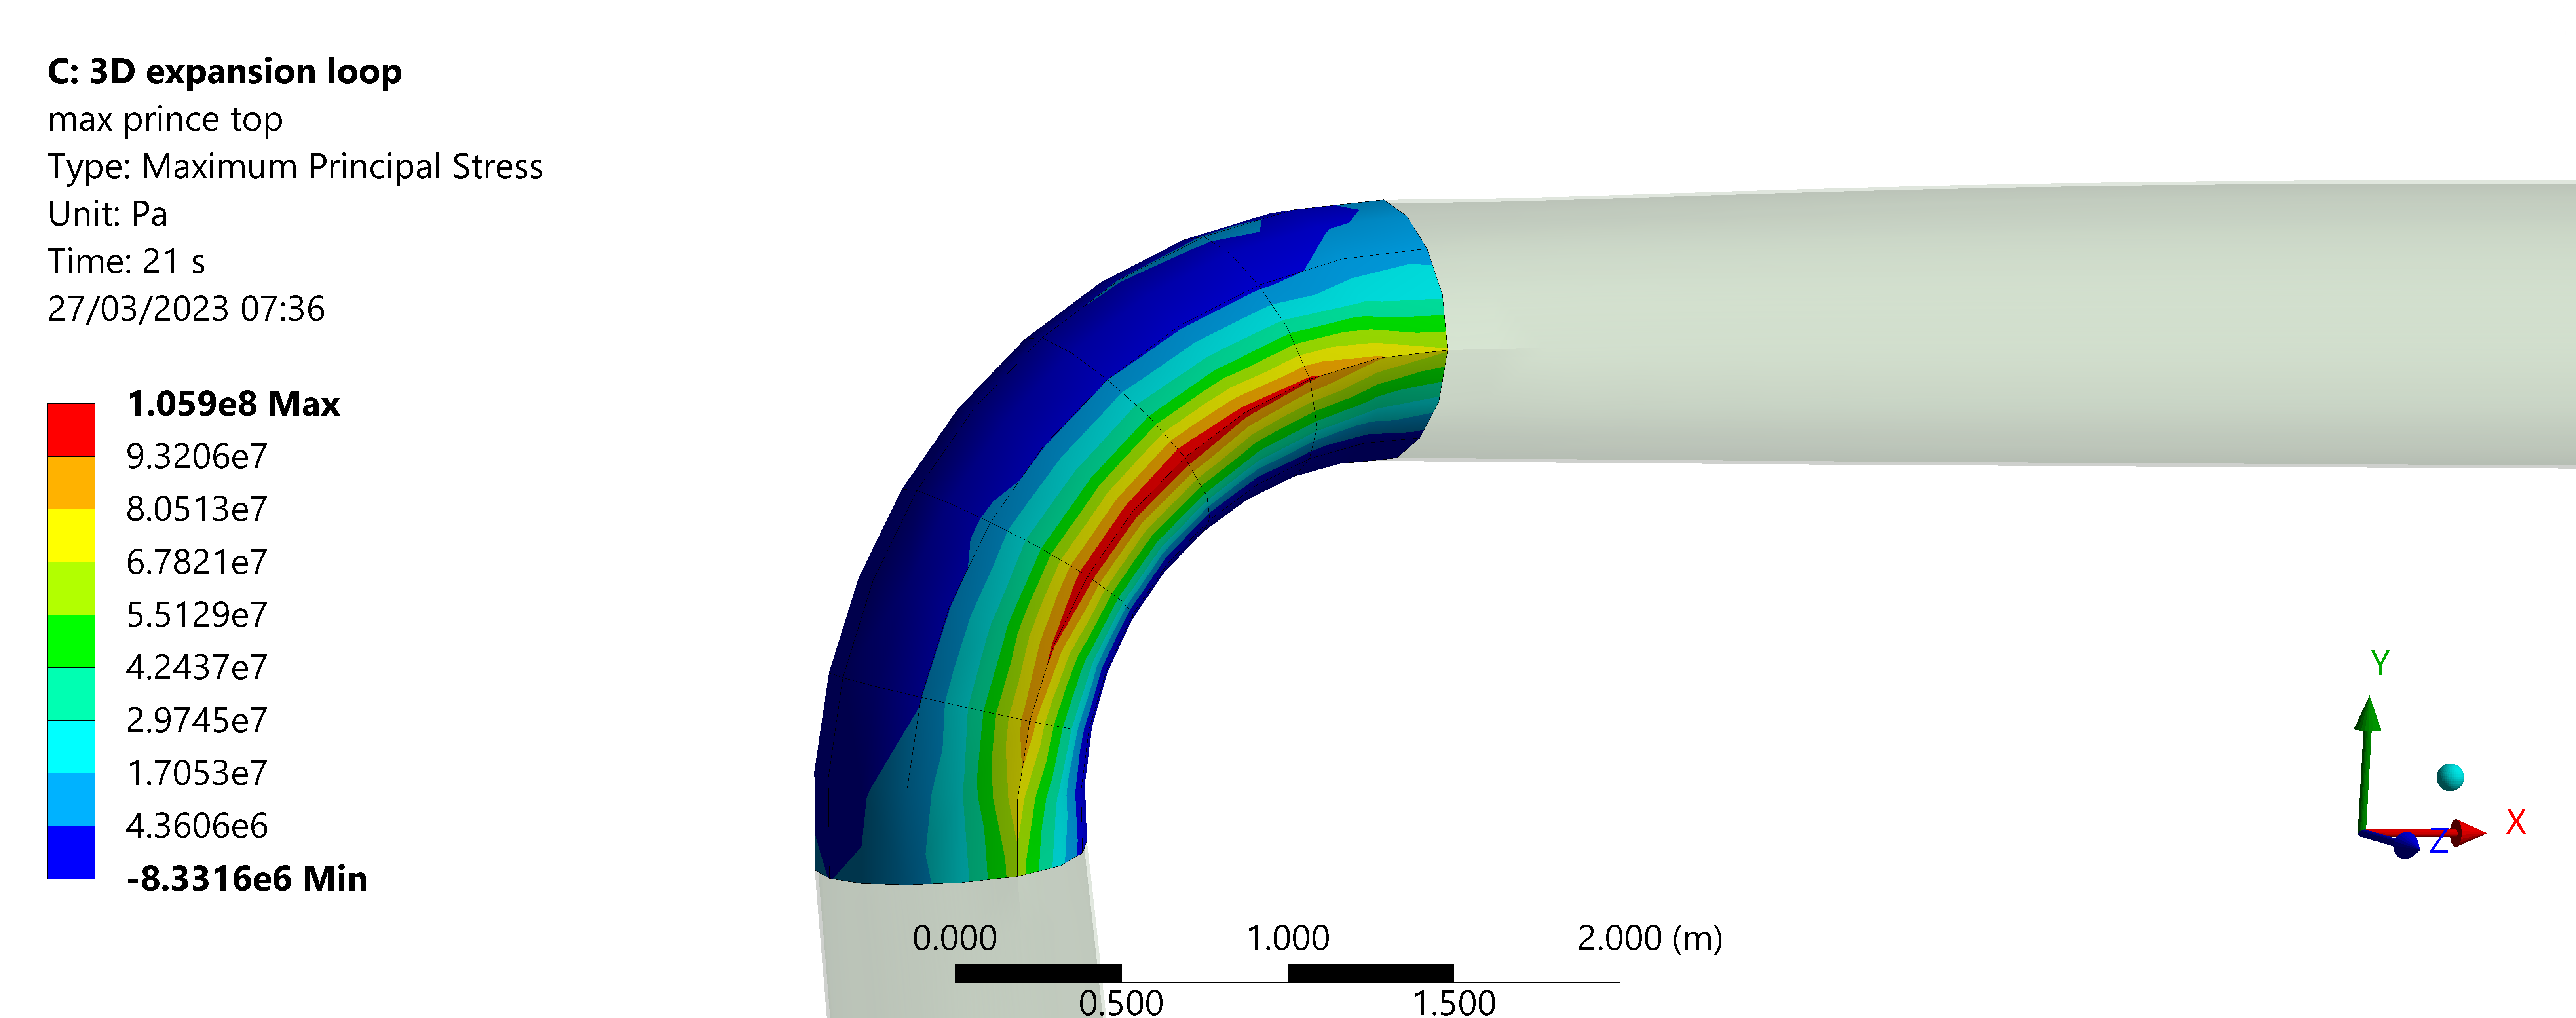
\includegraphics[width = 0.8\textwidth]{img/part2c-1.png}
    \caption{ANSYS maximum principal stress contour plot at time step 21, $T-T_0 = \SI{218}{\degree C}$, bottom pipe bend.}
    \label{part2c3}
\end{figure}
\begin{figure}[H]
    \centering
    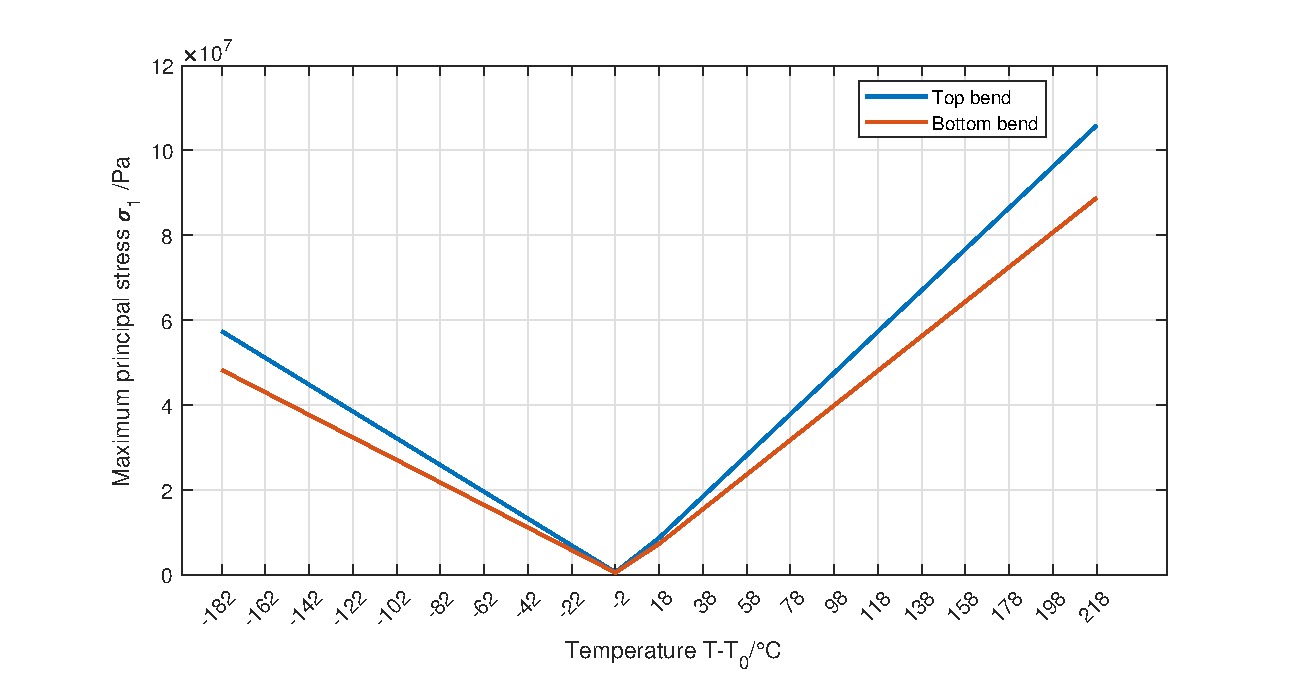
\includegraphics[width = \textwidth]{img/part2ci.eps}
    \caption{Plot to show maximum principal stress $\sigma_1$ of pipe bends.}
    \label{part2c1}
\end{figure}
\begin{figure}[H]
    \centering
    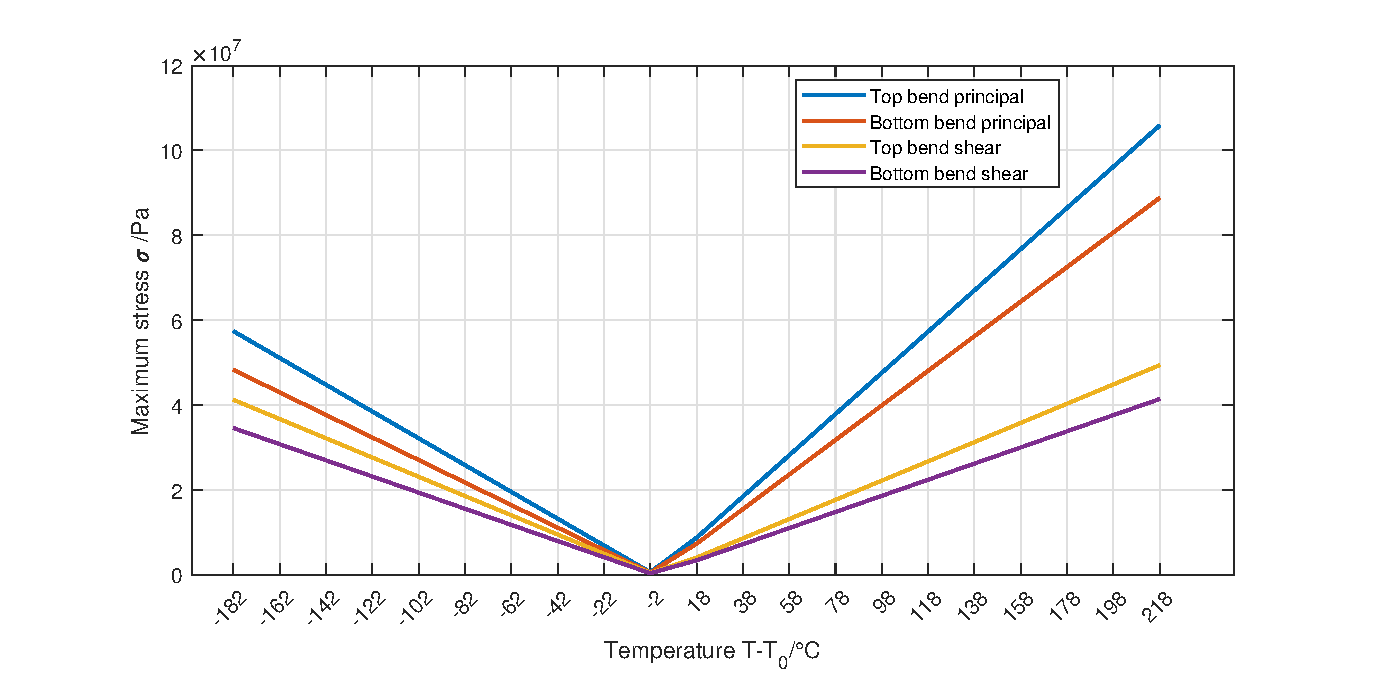
\includegraphics[width = \textwidth]{img/part2cii.eps}
    \caption{Plot to show maximum principal and shear stress of pipe bends.}
    \label{part2c2}
\end{figure}
\subsection{Comparison of numerical results}
The numerical results from each section show that straight sections of pipe have significantly more stress than those with a loop. We see that in the 3D simulation of a straight pipe, our maximum stress is approximately \SI{-5e8}{\pascal}. In comparison our 3D expansion loop has a maximum stress of \SI{1e8} in a comparatively small region at the pipe bend. The rest of the pipe has a much lower stress overall, as can be seen from the 1D simulation; 1 order of magnitude lower approximately. This shows that expansion loops are an effective tool in reducing overall pipe stress over a given span.

The practical implications of including an expansion loop in a pipework design are numerous. The first and major design implication is the extra space required for an expansion loop, requiring much more consideration, especially in complex scenarios with a high density of pipework. This coursework has considered a relatively simple design for an expansion loop, only extending in-plane. However, expansion loops can take up larger volumes if they are designed with two loops (one extending in-plane and one extending out of plane). Yavuz provides the rationale for design requirements and recommendations for expansion loop designs in the Oil and Gas industry, mentioning that expansion loops extending in all three dimensions prevent possible conflicts to other lines \cite{expansionLoop1}. However, such complexity comes at a cost (in many forms). First, we must consider that more complex loops require more complex supports and these must be modelled beforehand increasing development time and cost. Second, more complex loops require more material and bracing which has a physical and monetary cost associated with it. Third, the maintenance of such a loop must also be considered as more complex piping and bracing requires thorough checks and potentially repairs over the course of its lifetime. Another consideration is the overall pressure drop in the system as a result of the increase in the total length of the pipe. This effect can be mitigated by carefully selecting the length and configuration of the expansion loop, as well as the material properties of the piping and the fluid being transported.

In the UK, all piping must follow a set of codes as outlined by the Health and Safety Executive (HSE). Specifically, the HSE outlines via a Technical Measures Document the specific codes that must be followed for design work involving pipework \cite{hseCode1}. ASME B31.3 is the code  that outline the design, construction, operation, and maintenance requirements for piping systems, specifically for Process Piping \cite{asmeb31}. Other codes of interest are the Pressure Systems Safety Regulations 2000, which outlines general safety regulations around pipework and the California Plumbing Code 2022, which outlines specific geometry and equations for expansion loop design \cite{hseCode2,caliCode}.

In ASME B31.3, the maximum allowable stress takes the following form in the thermal expansion case:
\begin{equation}
    S = f\left[\left(\left(\frac{1.25}{E}\right)\times \left(S_c + S_h\right)\right)- S_E\right]
\end{equation}
where $f$ is the stress range factor, $E$ is Young's Modulus, $S_c$ is the basic allowable stress at minimum metal temperature, $S_h$ is the basic allowable stress at maximum metal temperature and $S_E$ is the code stress. $S_E$ is defined as:
\begin{equation}
    S_E = \sqrt{S^2_b + 4S_t^2}
\end{equation}
where $S_b$ is the bending stress and $S_t$ is the torsional stress. To make a comparison, the California Plumbing codes utilise a different methodology, giving specifications to the lengths of different parts of the expansion loop. The California Plumbing code state that the minimum length of expansion arms $LB$ shall be calculated using the following equation:
\begin{equation}
    LB = C\times \sqrt{D \times \Delta L}
\end{equation}
where $C$ is the material constant, $D$ is the nominal outside diameter of tubing and $\Delta L$ is the thermal expansion length. Hence:
\begin{equation}
    LB = W + \left(2\times H\right)
\end{equation}
where $W = LB/5$ is the length of the top part of the loop, and $H = 2W$ is the length of the vertical sections of the loop (as specified in the earlier geometry used for expansion loop analysis).

Shehadeh \textit{et al} conducts `an optimization analysis concerning the expansion loop dimensions and the number of supports without compromising on the safety of piping. The design approach is conducted as per the guidelines of ASME B31.3 (Process Piping) code.' The analysis results show that through a physics based approach, expansion loops can be well designed to minimise material and cost, whilst adhering to ASME B31 codes, rather than through empirical means, which is the norm in industry \cite{Shehadeh}.

The practical implications of including an expansion loop in a pipework design are significant and require careful consideration of various factors, including material selection, installation and maintenance, system compatibility, and cost considerations. However, by following industry standards and best practices, the inclusion of this expansion loop can greatly improve the reliability and longevity of the piping system, making it a worthwhile investment in many cases.
\subsection{1D pipe model and consequences of increasing length L1 and effect on maximum pipe stress}
ANSYS was used to construct two expansion loops with $L_1 = \SI{10}{\meter}$ and $L_1 = \SI{50}{\meter}$. The results are shown in the following Figures.
\begin{figure}[H]
    \centering
    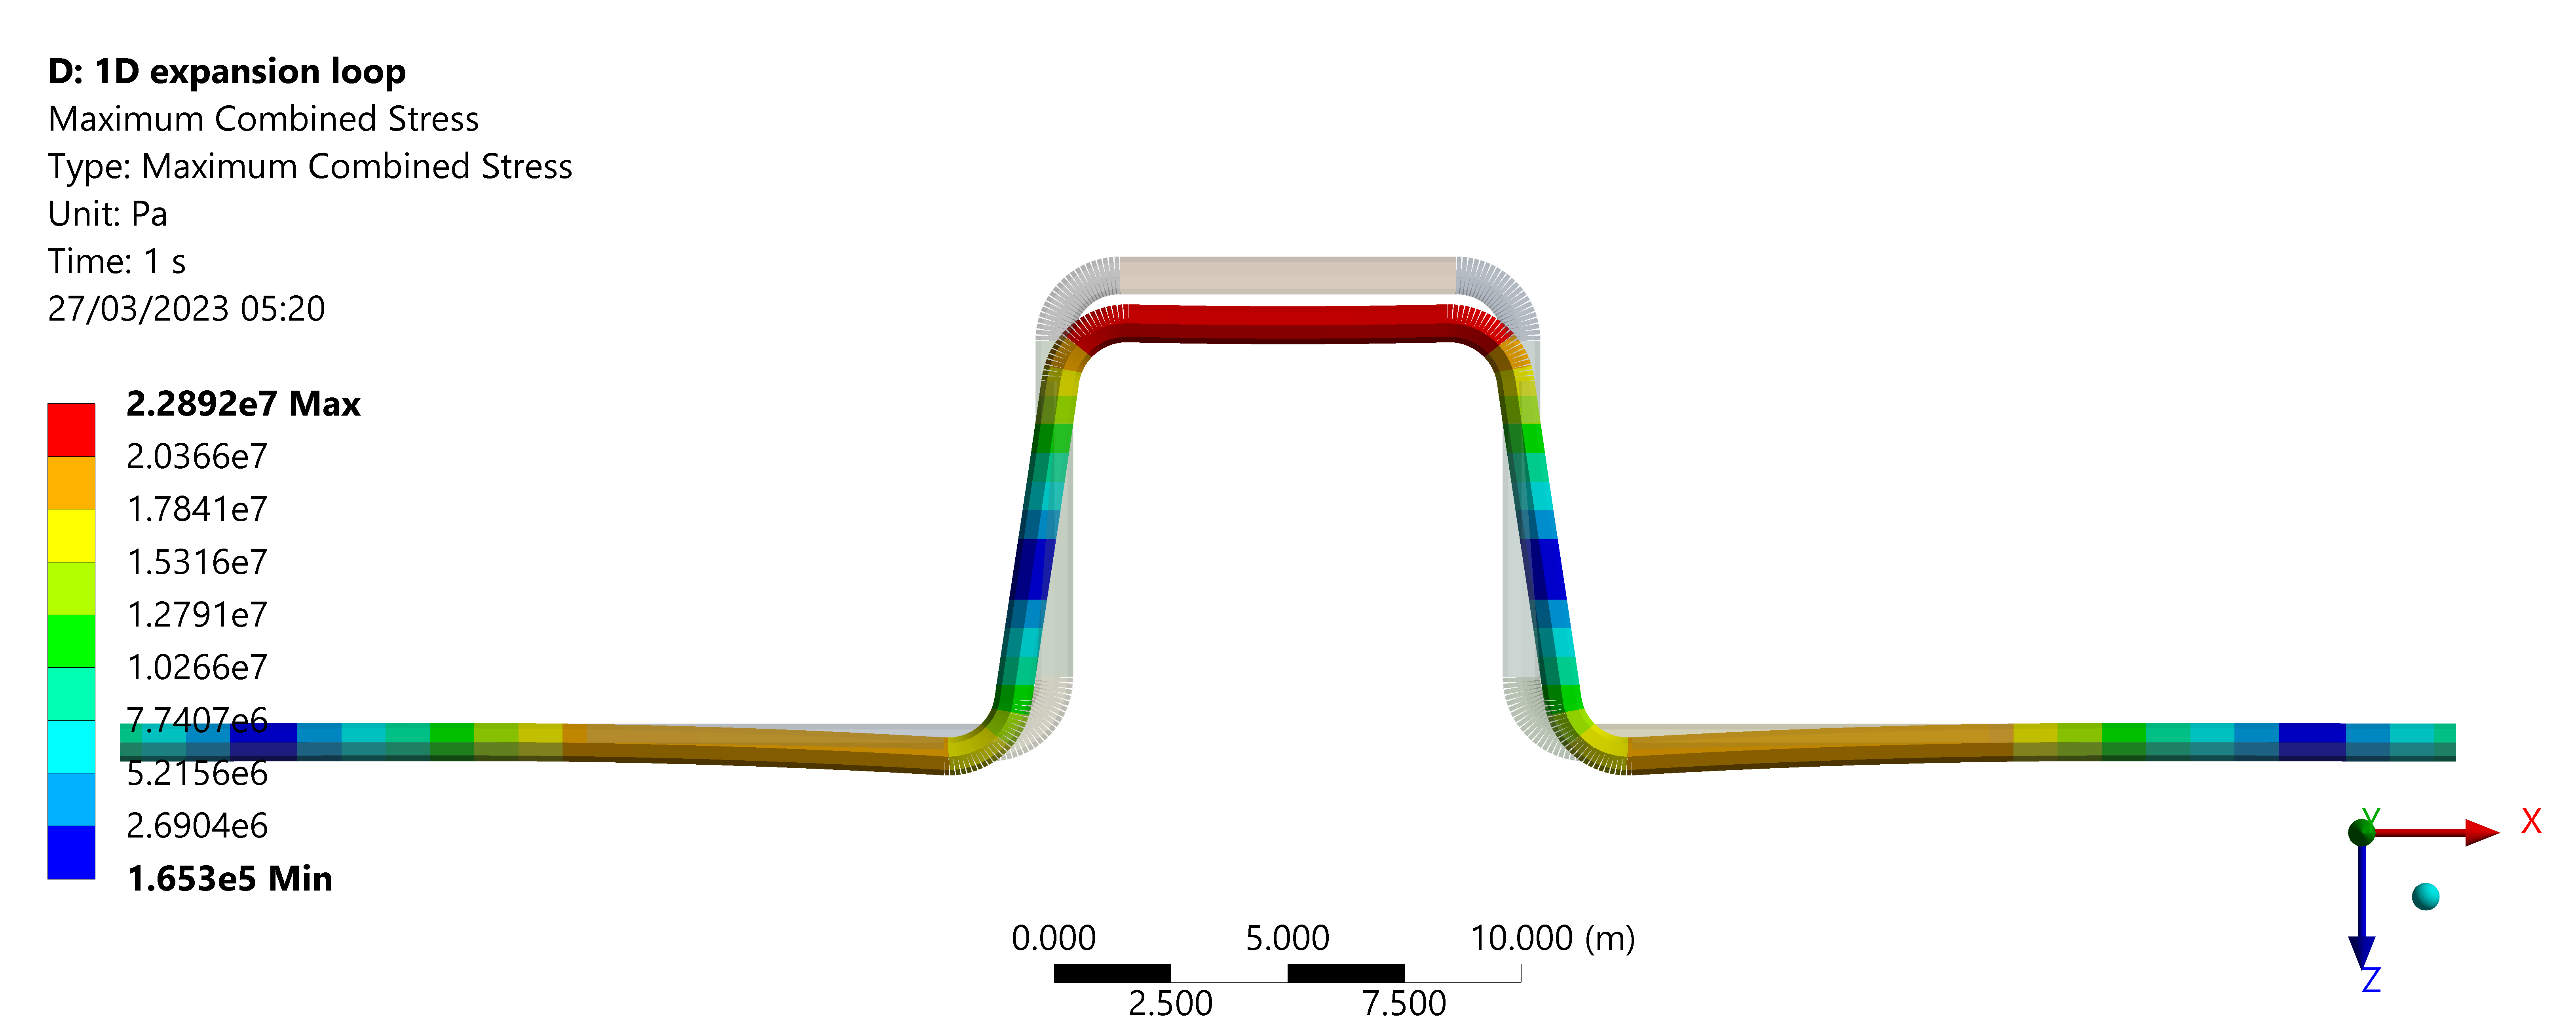
\includegraphics[width = \textwidth]{img/part2e-1.png}
    \caption{ANSYS results from 1D expansion loop $L_1 = \SI{10}{\meter}$, time step 1, $T = \SI{-160}{\degree C}$, maximum combined stress.}
\end{figure}
\begin{figure}[H]
    \centering
    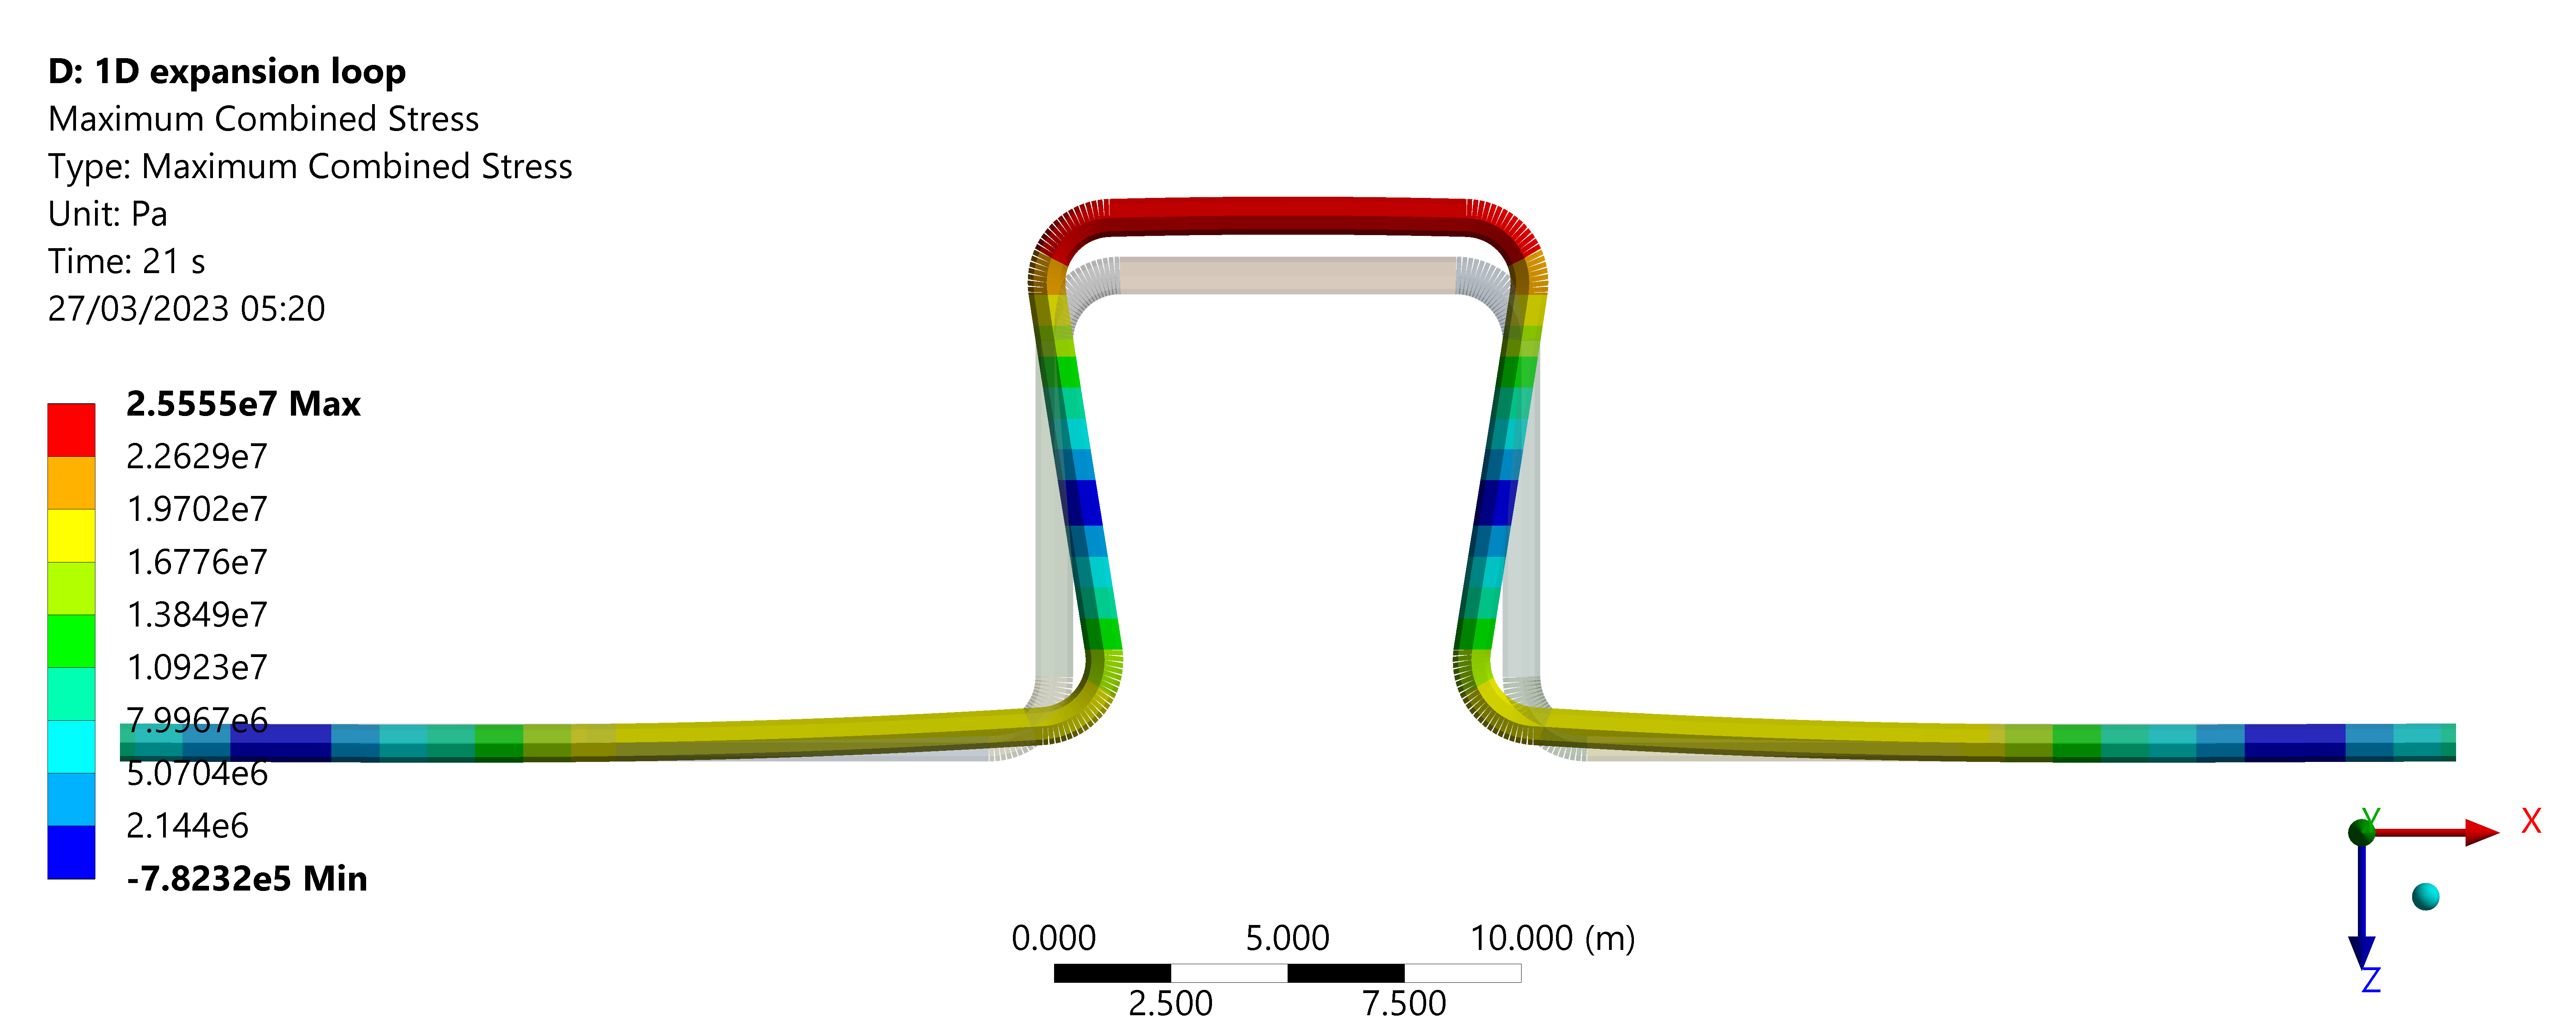
\includegraphics[width = \textwidth]{img/part2e-2.png}
    \caption{ANSYS results from 1D expansion loop $L_1 = \SI{10}{\meter}$, time step 21, $T = \SI{240}{\degree C}$, maximum combined stress.}
\end{figure}
\begin{figure}[H]
    \centering
    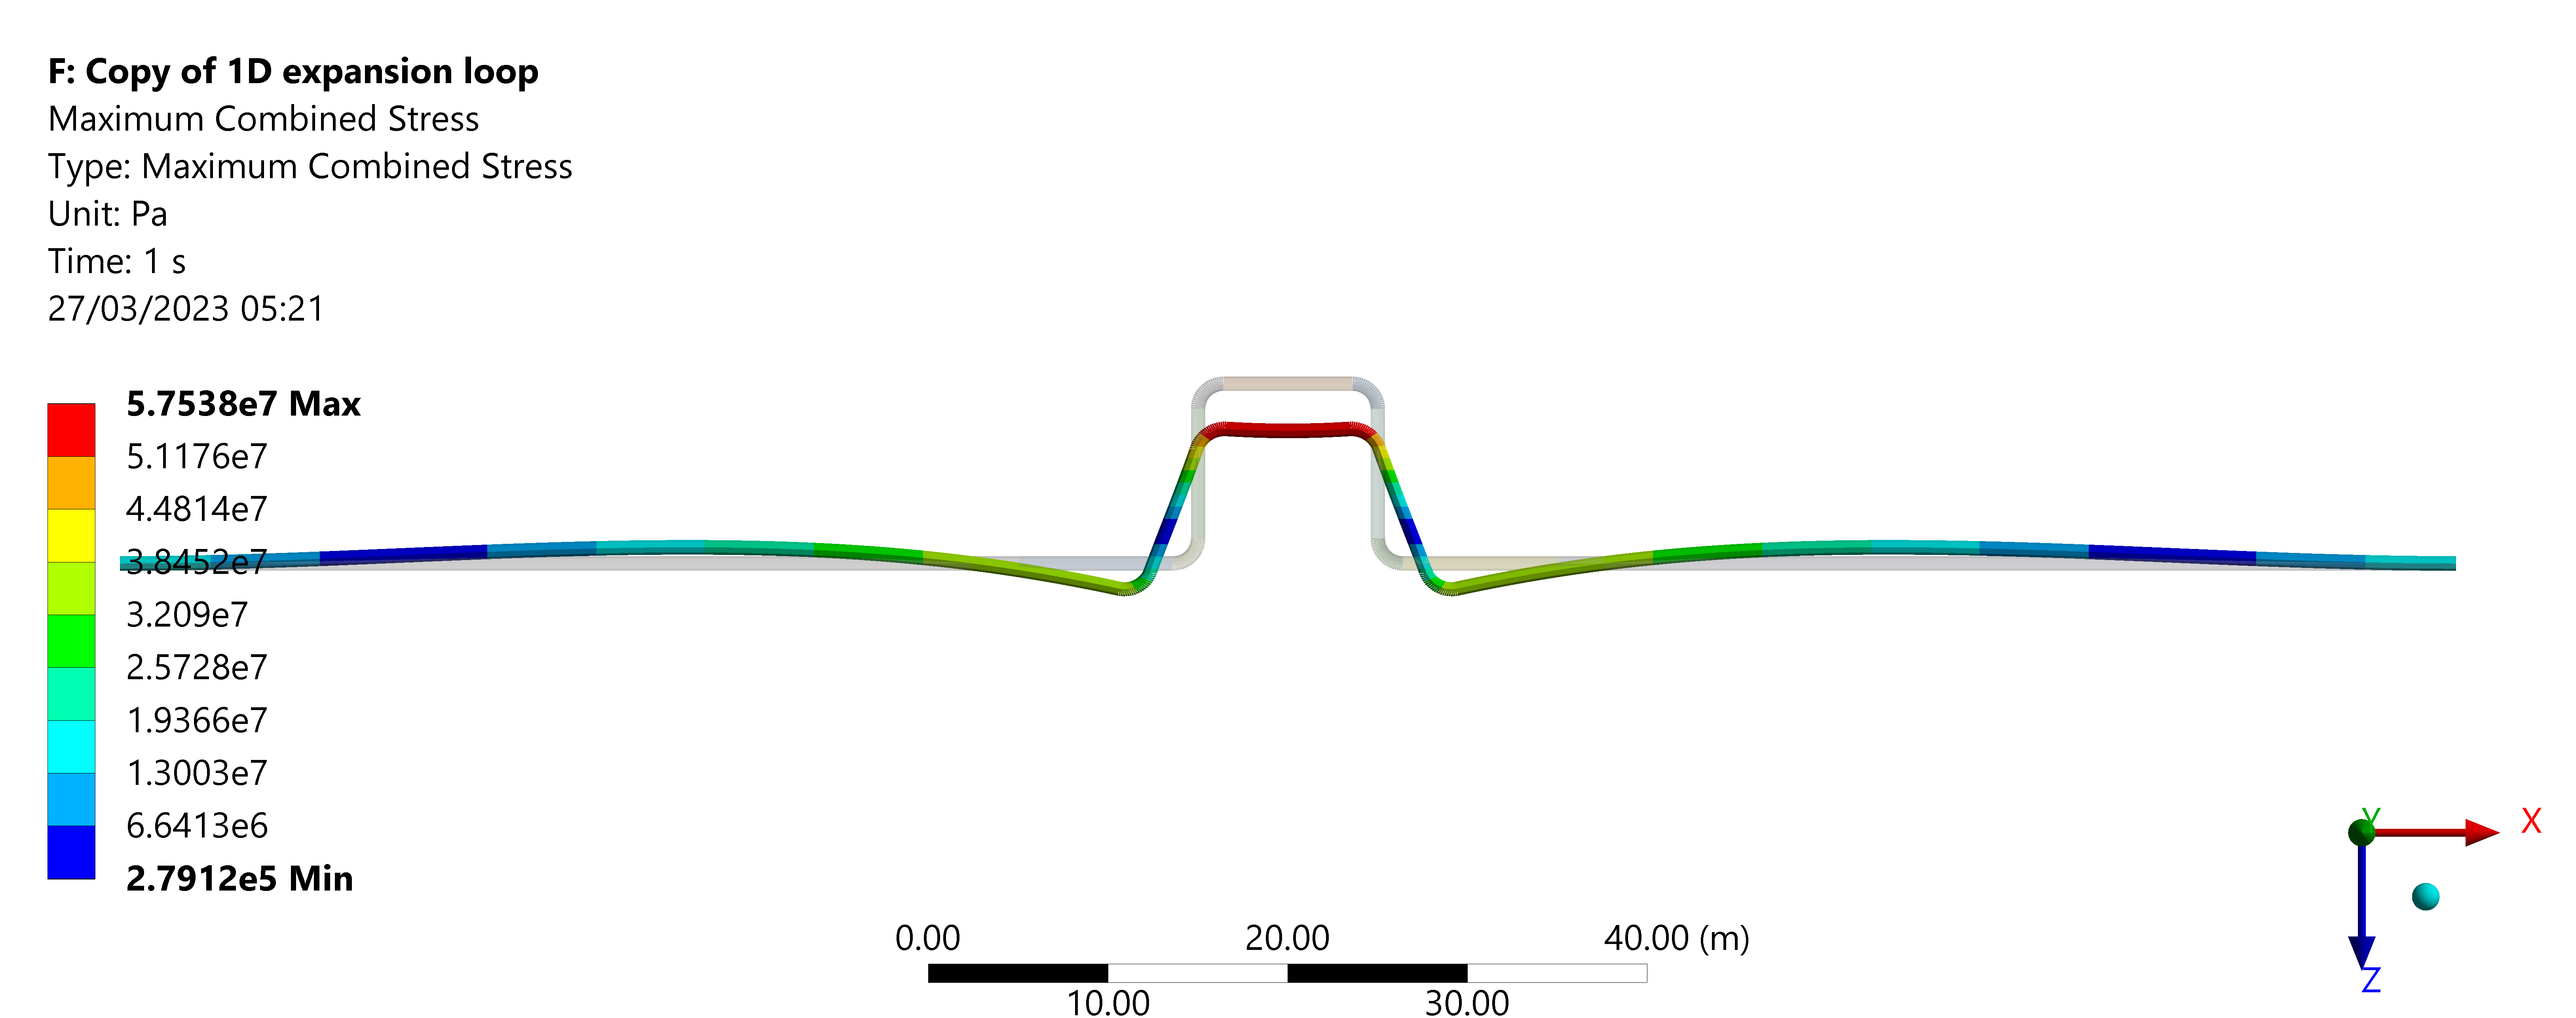
\includegraphics[width = \textwidth]{img/part2e-3.png}
    \caption{ANSYS results from 1D expansion loop $L_1 = \SI{50}{\meter}$, time step 1, $T = \SI{-160}{\degree C}$, maximum combined stress.}
\end{figure}
\begin{figure}[H]
    \centering
    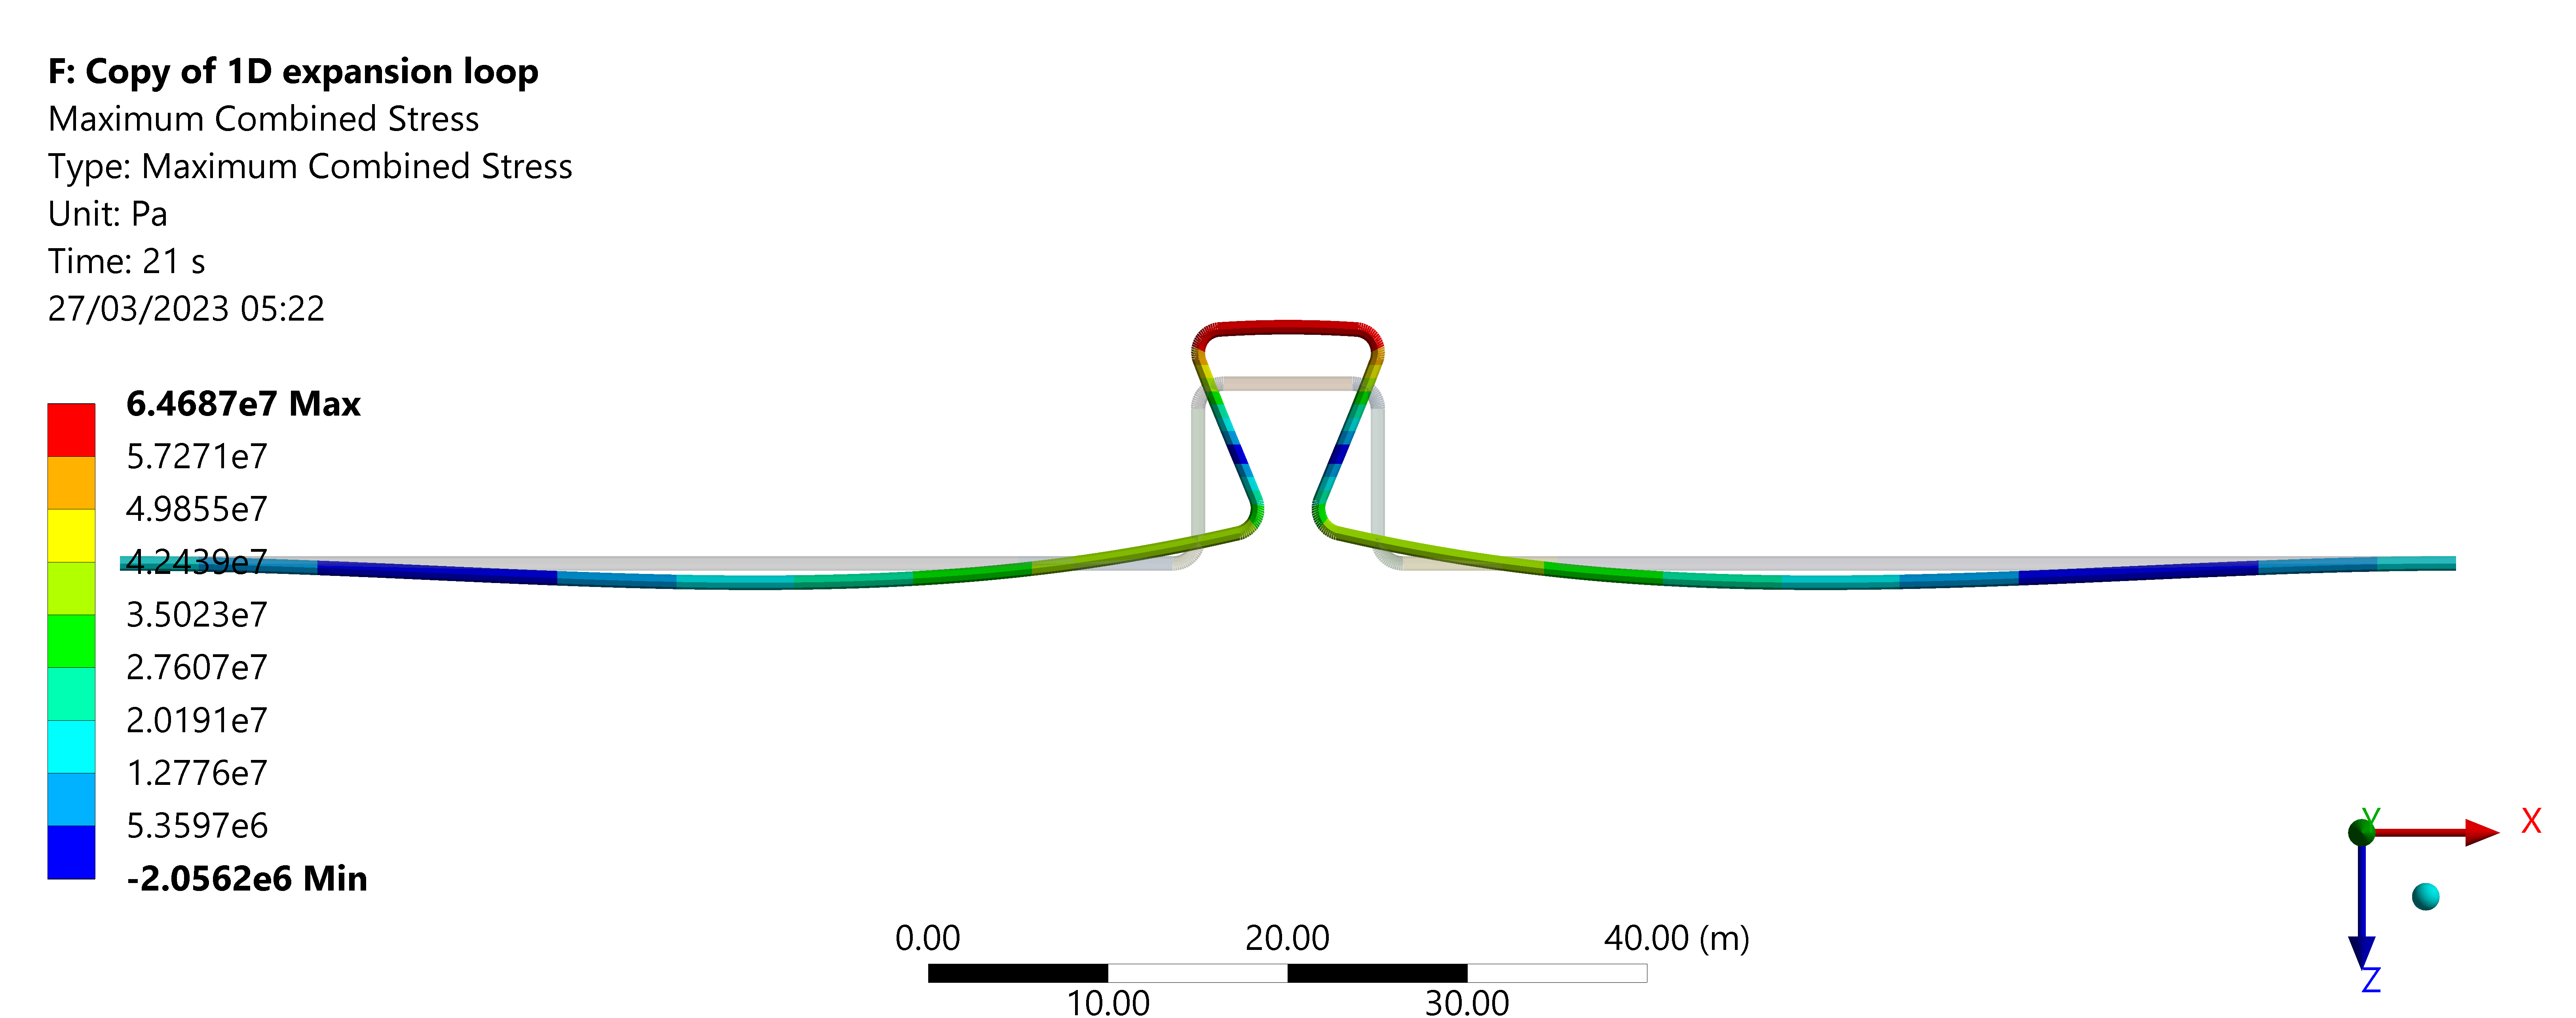
\includegraphics[width = \textwidth]{img/part2e-4.png}
    \caption{ANSYS results from 1D expansion loop $L_1 = \SI{50}{\meter}$, time step 21, $T = \SI{240}{\degree C}$, maximum combined stress.}
\end{figure}
\begin{figure}[H]
    \centering
    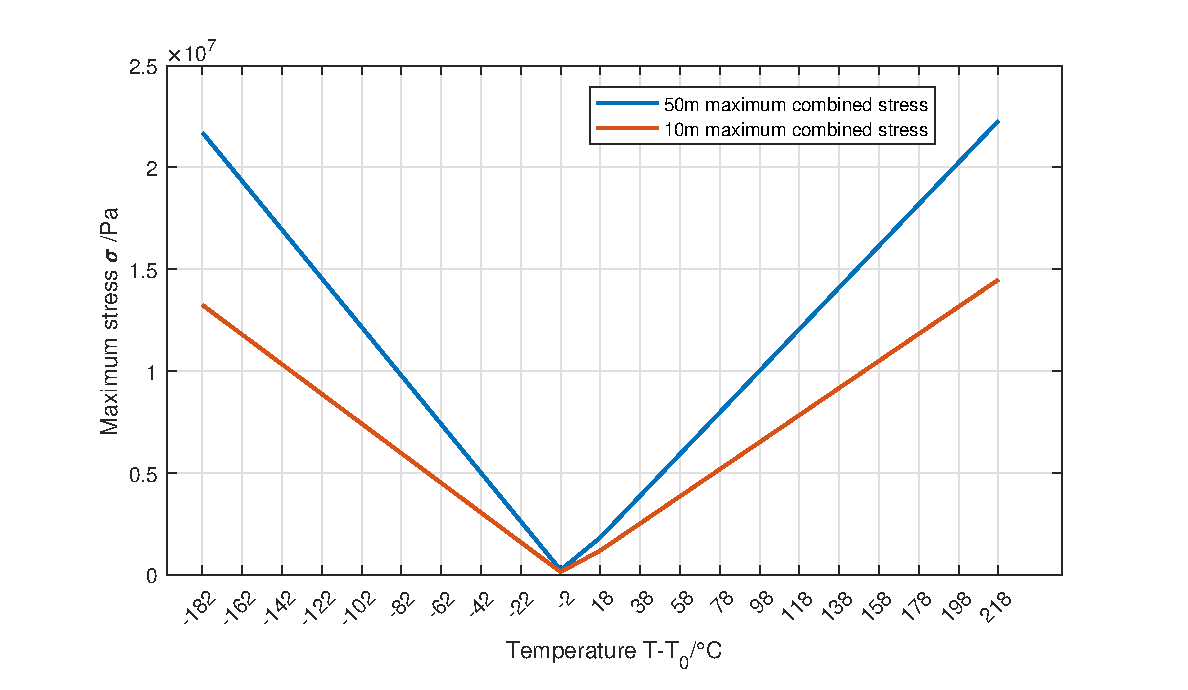
\includegraphics[width = \textwidth]{img/part2ei.eps}
    \caption{Maximum combined stress of $L_1$ \SI{50}{\meter} and \SI{10}{\meter} expansion loops.}
\end{figure}
The results show that as $L_1$ increases, the maximum combined stress increases in all cases. This is due to the fact that there is more material that is subject to contraction/expansion. Due to the constraint at the boundary between $L_1$ and $L_2$, we see higher stresses due to higher deformation in the loop.

Increasing the size of $L_1$ may also require changes to the design of the supports used to hold the loop in place. For larger loops, additional supports may be required to ensure that the loop remains stable and does not experience excessive stress, deflection or deformation from the thermal expansion of the material. This can also have implications for the overall safety and reliability of the system, and may require additional design considerations to ensure that the system remains within safe operating limits.